\documentclass{article}
\usepackage{graphicx}

\title{Tugas Database 2}
\begin{figure}
    \begin{center}
        
\includegraphics[width=6cm]{poltekpos.jpg}
    \end{center}
\end{figure}
\author{Annisa Khairani Febrianti}
\date{1184071}

\begin{document}

\maketitle

\section{Cara Membuat Aplikasi Builder dari file Excel ke Oracle Apex}
\begin{enumerate}
    \item Buka aplikasi Oracle Apex terlebih dahulu
         \begin{figure}[h]
            \centerline{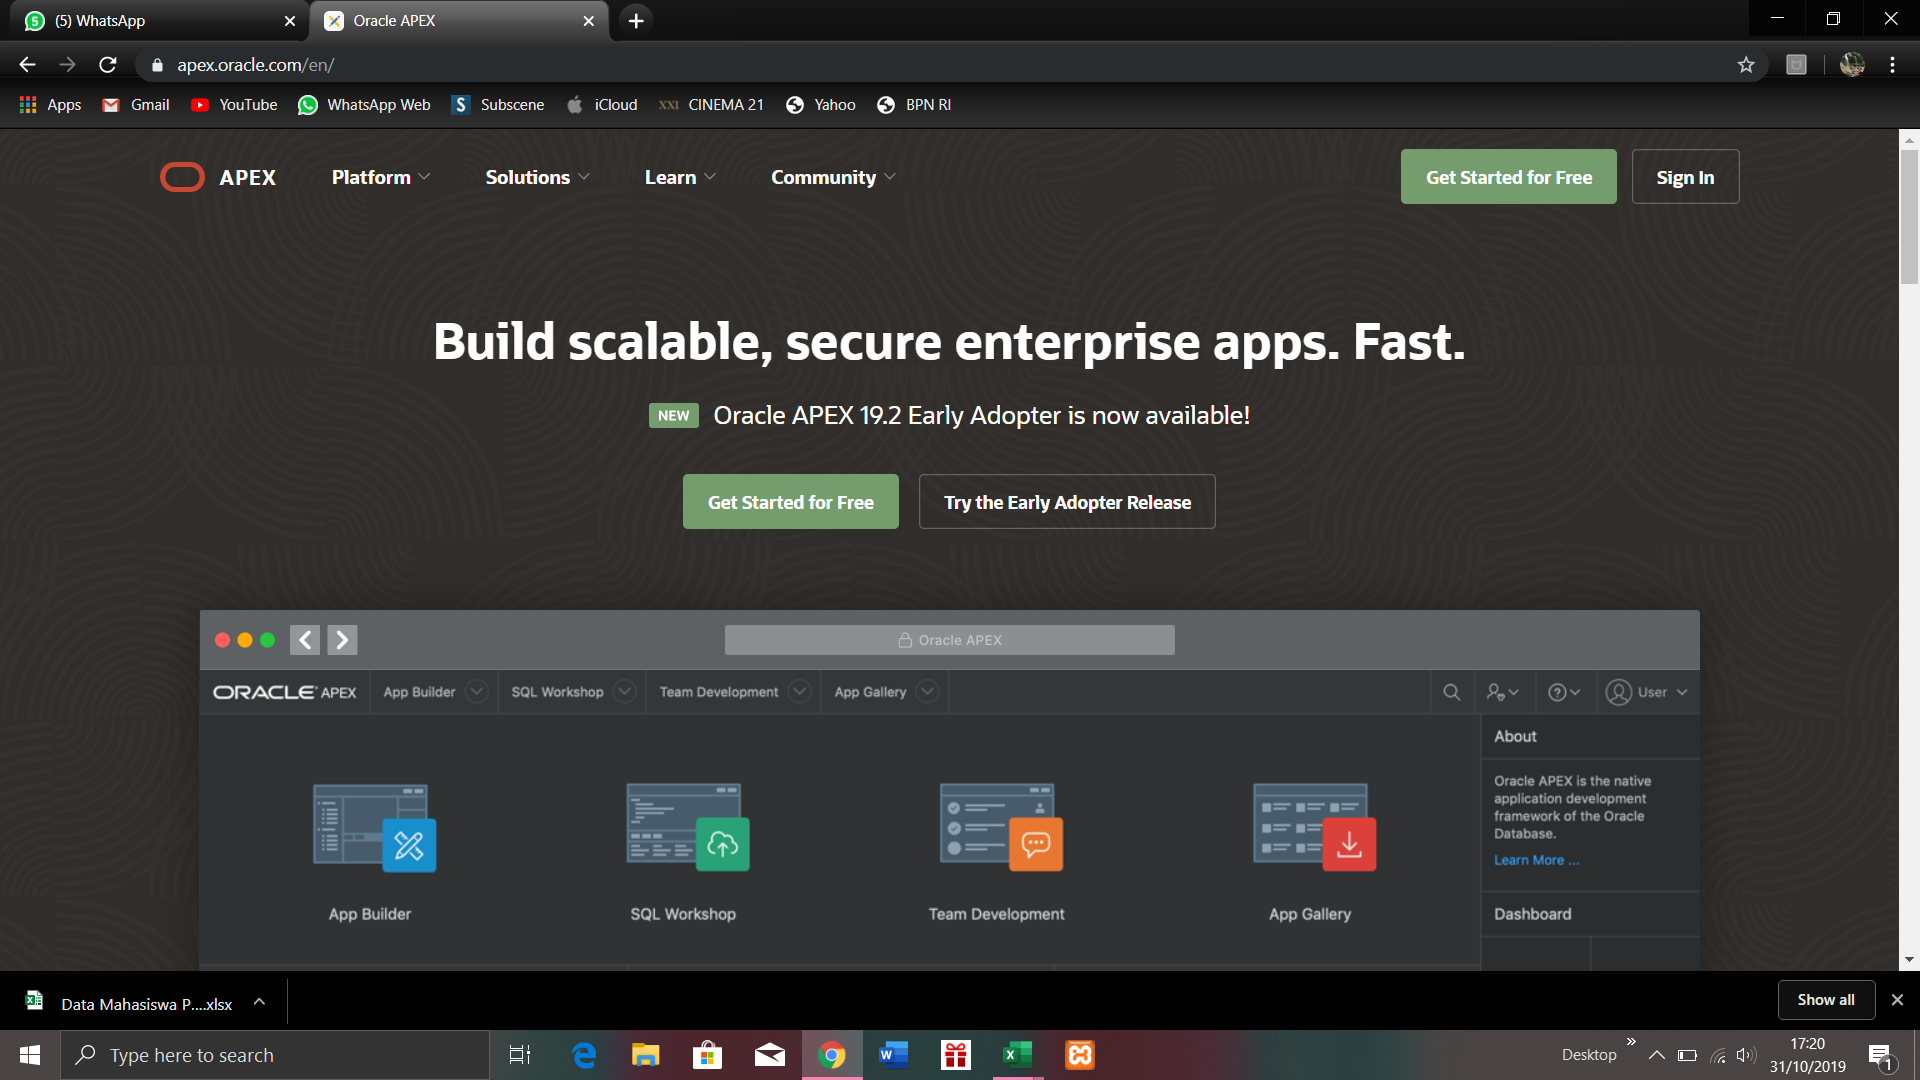
\includegraphics[width=8cm]{image/1.png}}
            \end{figure}
    \newpage \item Kemudian masukkan workspace,username,dan password
         \begin{figure}[h]
    \centerline{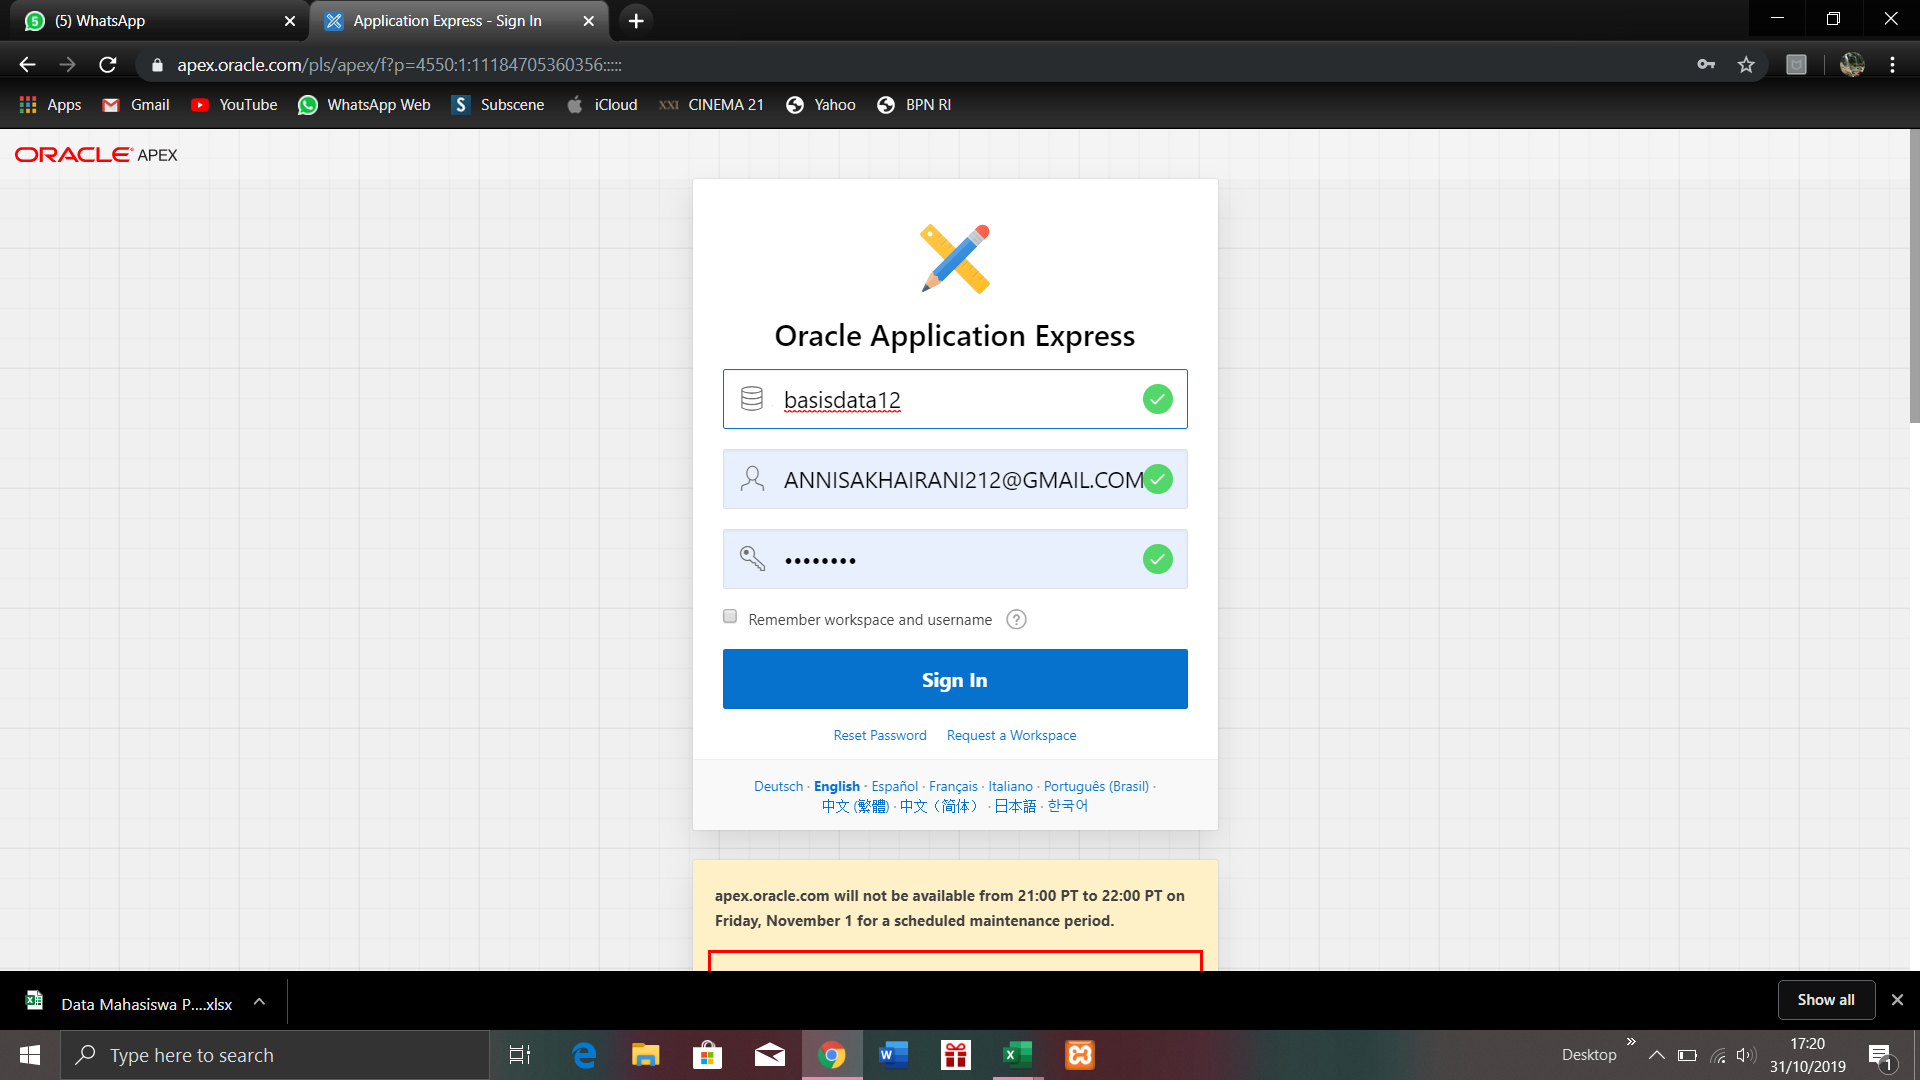
\includegraphics[width=8cm]{image/2.png}}
    \end{figure}
    \item Setelah selesai masukkan workspace,username,dan password kemudian akan muncul tampilan seperti gambar dibawah ini, kemudian kita pilih App Builder
         \begin{figure}[h]
            \centerline{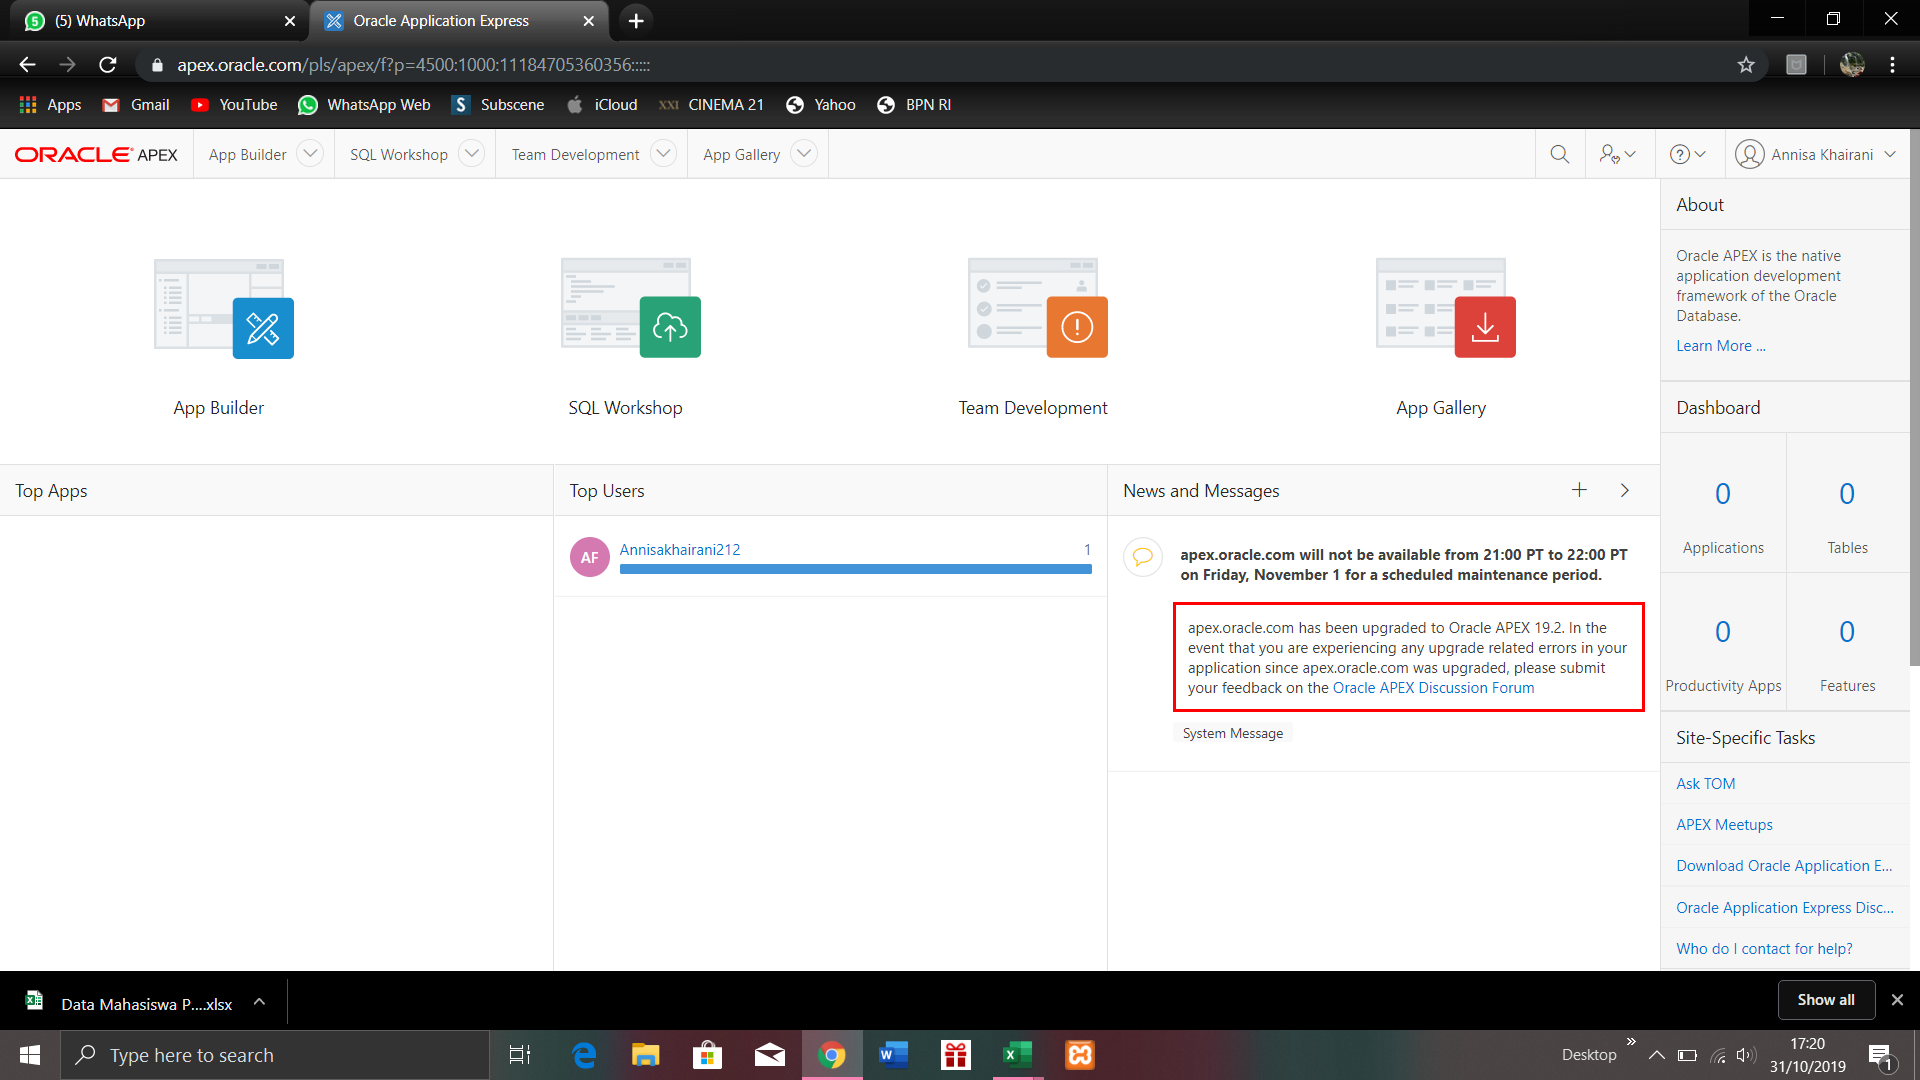
\includegraphics[width=6cm]{image/3.png}}
            \end{figure}
    \item Lalu kita pilih create
        \begin{figure}[h]
            \centerline{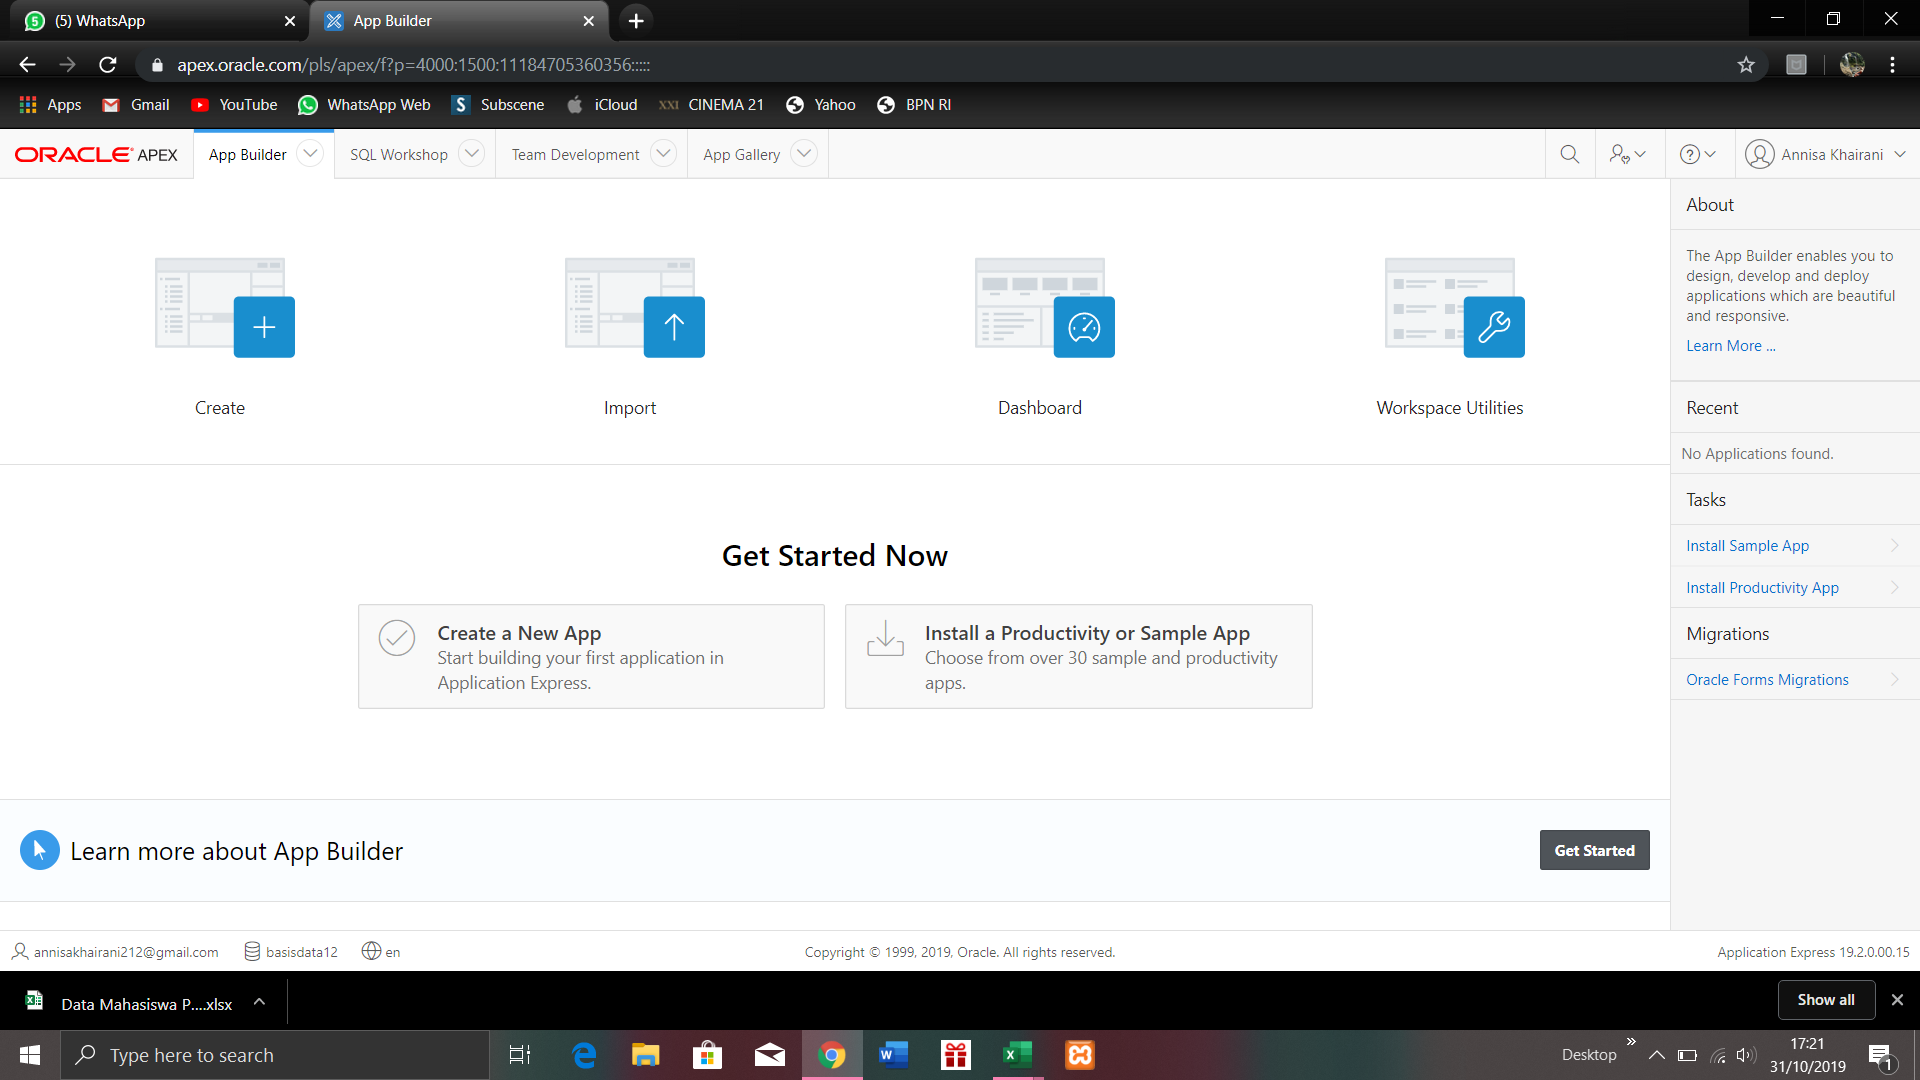
\includegraphics[width=8cm]{image/4.png}}
            \end{figure}
    \newpage \item Setelah itu kita pilih create, lalu kita pilih Form a file
        \begin{figure}[h]
            \centerline{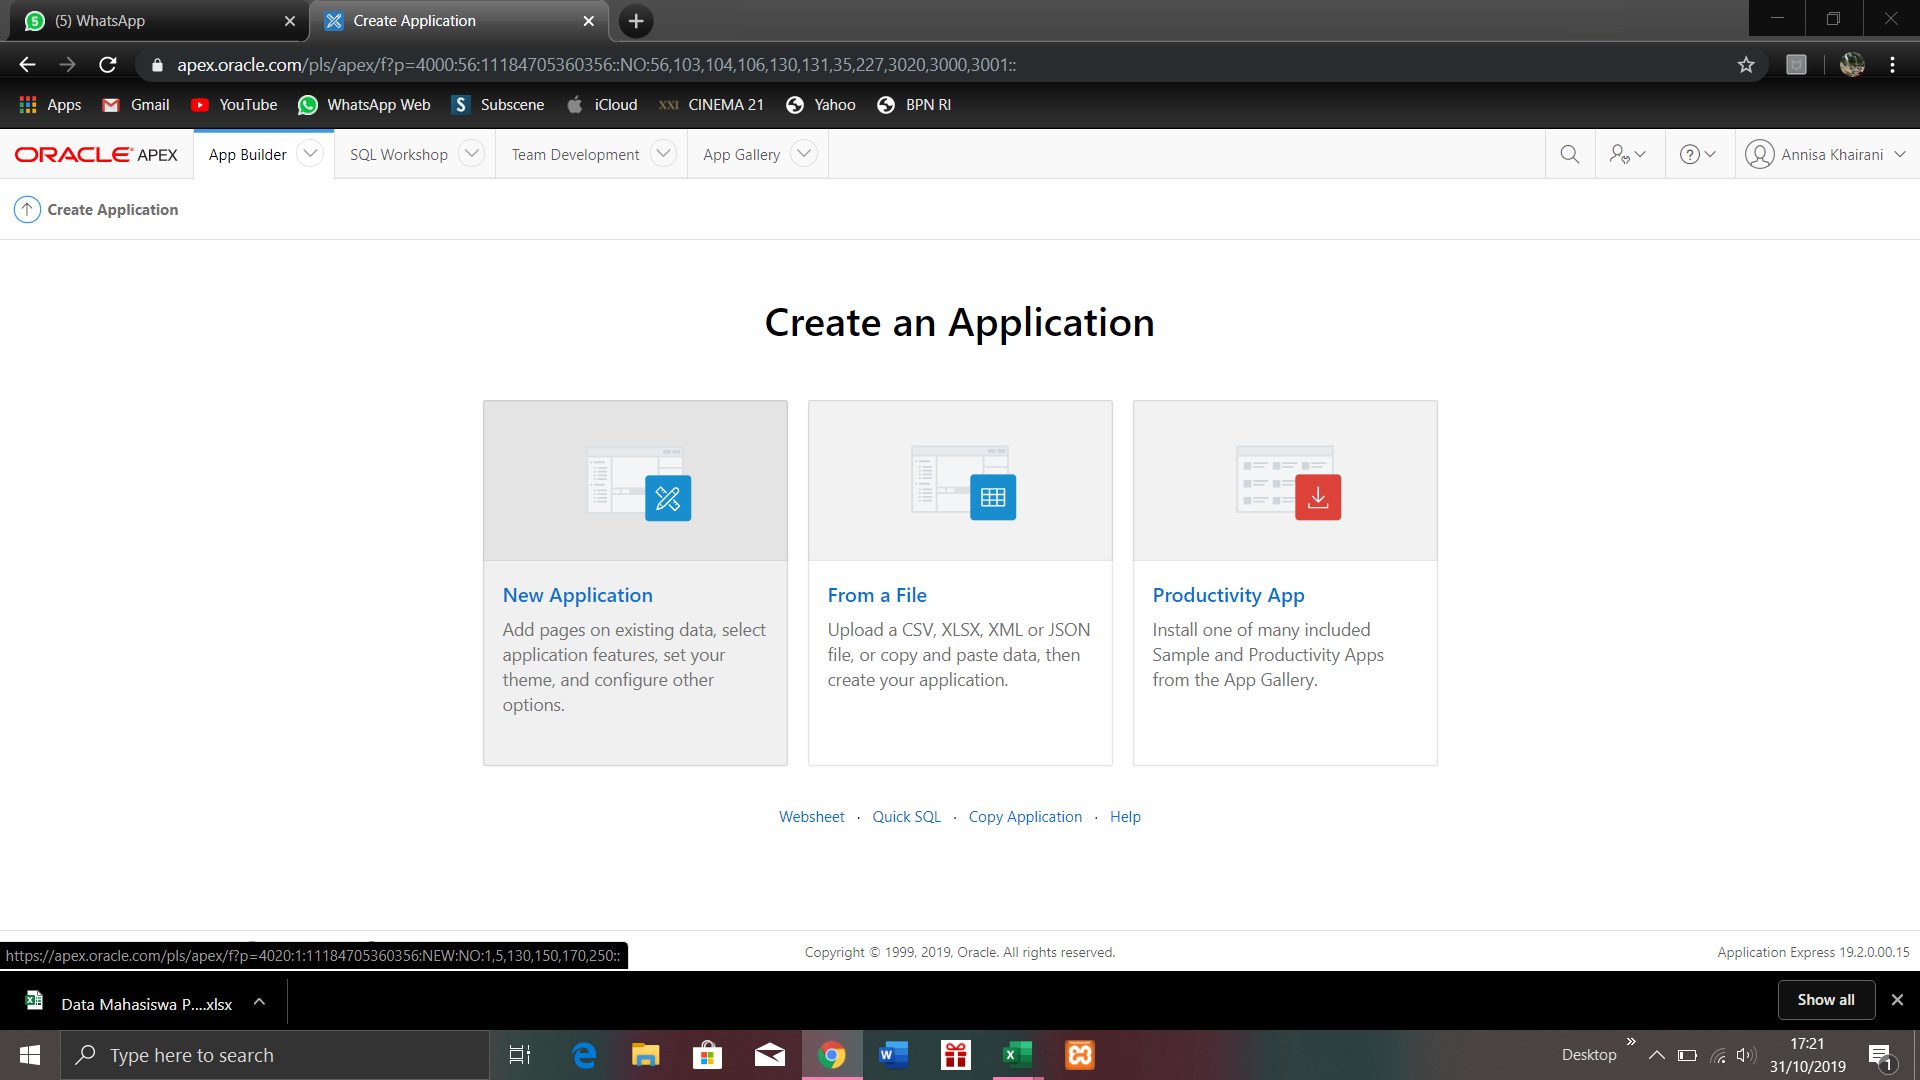
\includegraphics[width=8cm]{image/5.png}}
            \centerline{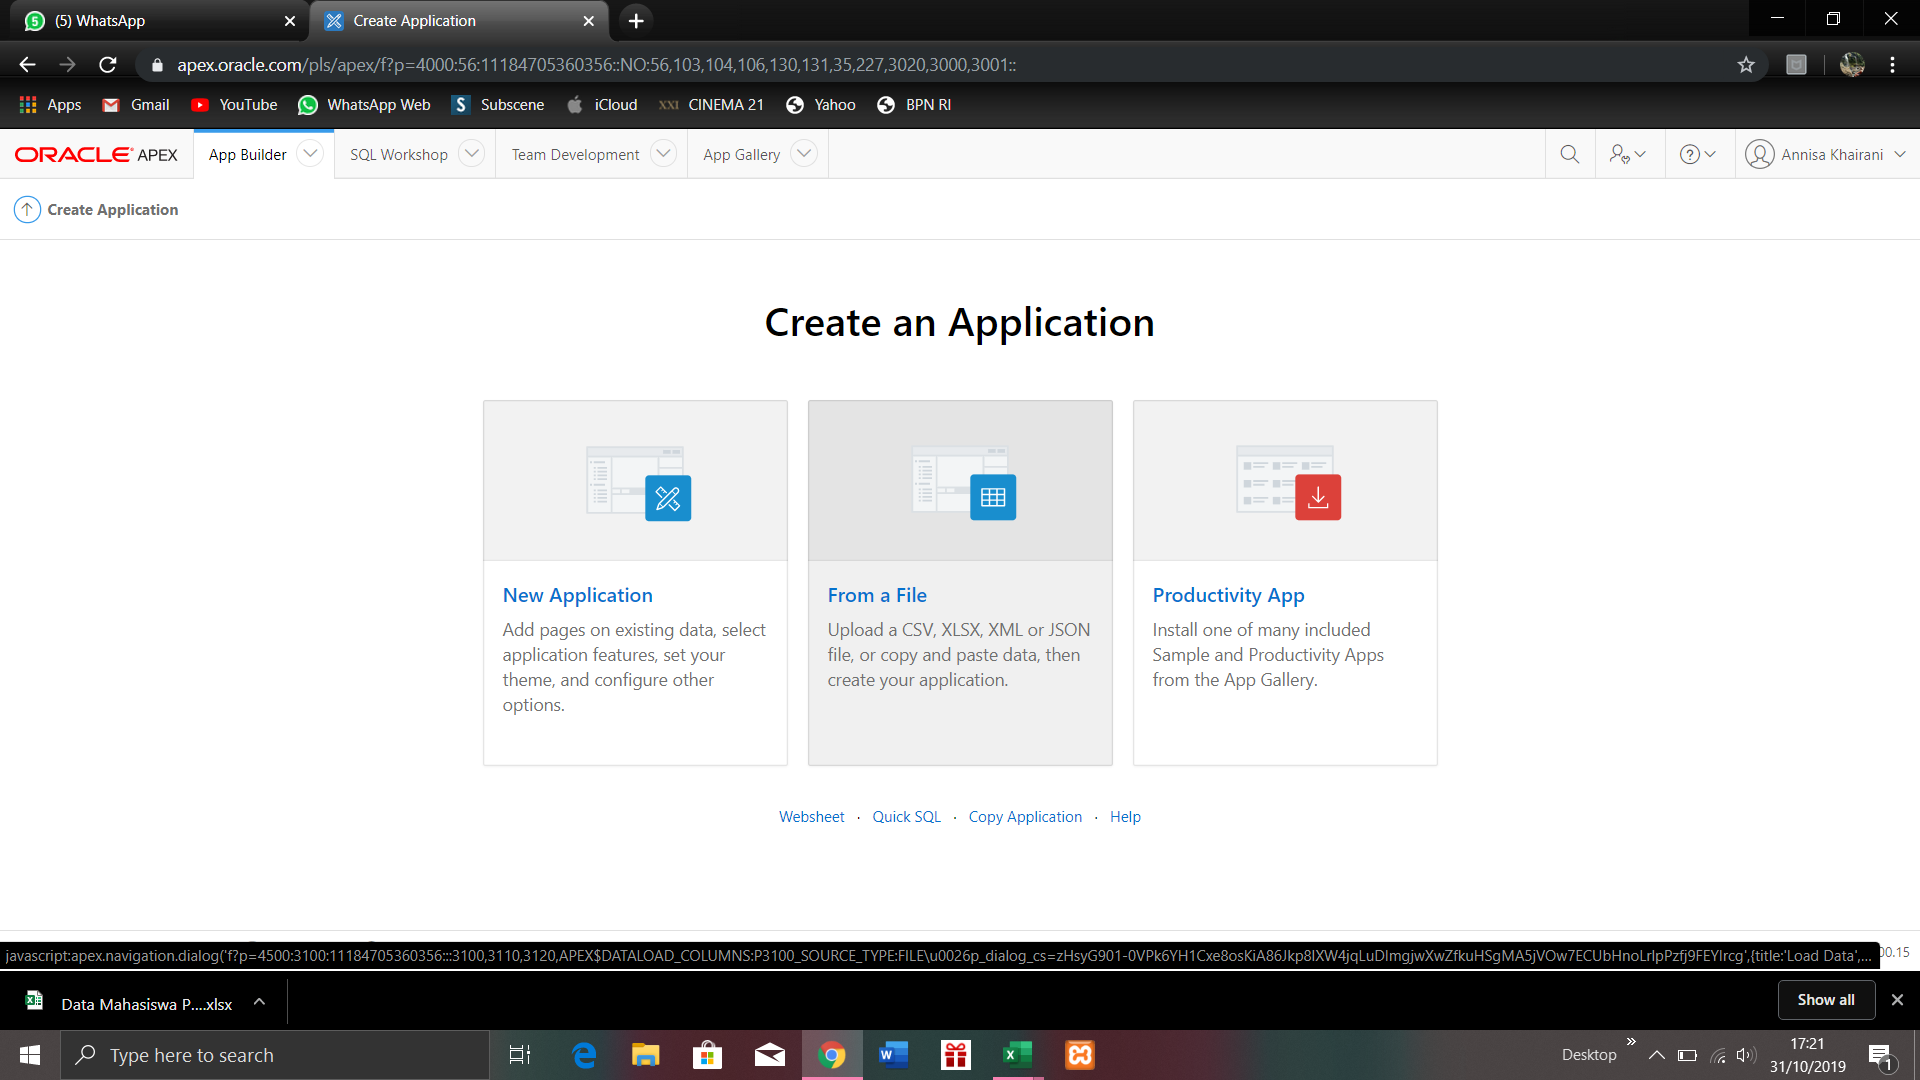
\includegraphics[width=8cm]{image/6.png}}
            \end{figure}
    \item Kemudian akan muncul tampilan seperti dibawah ini
        \begin{figure}[h]
           \centerline{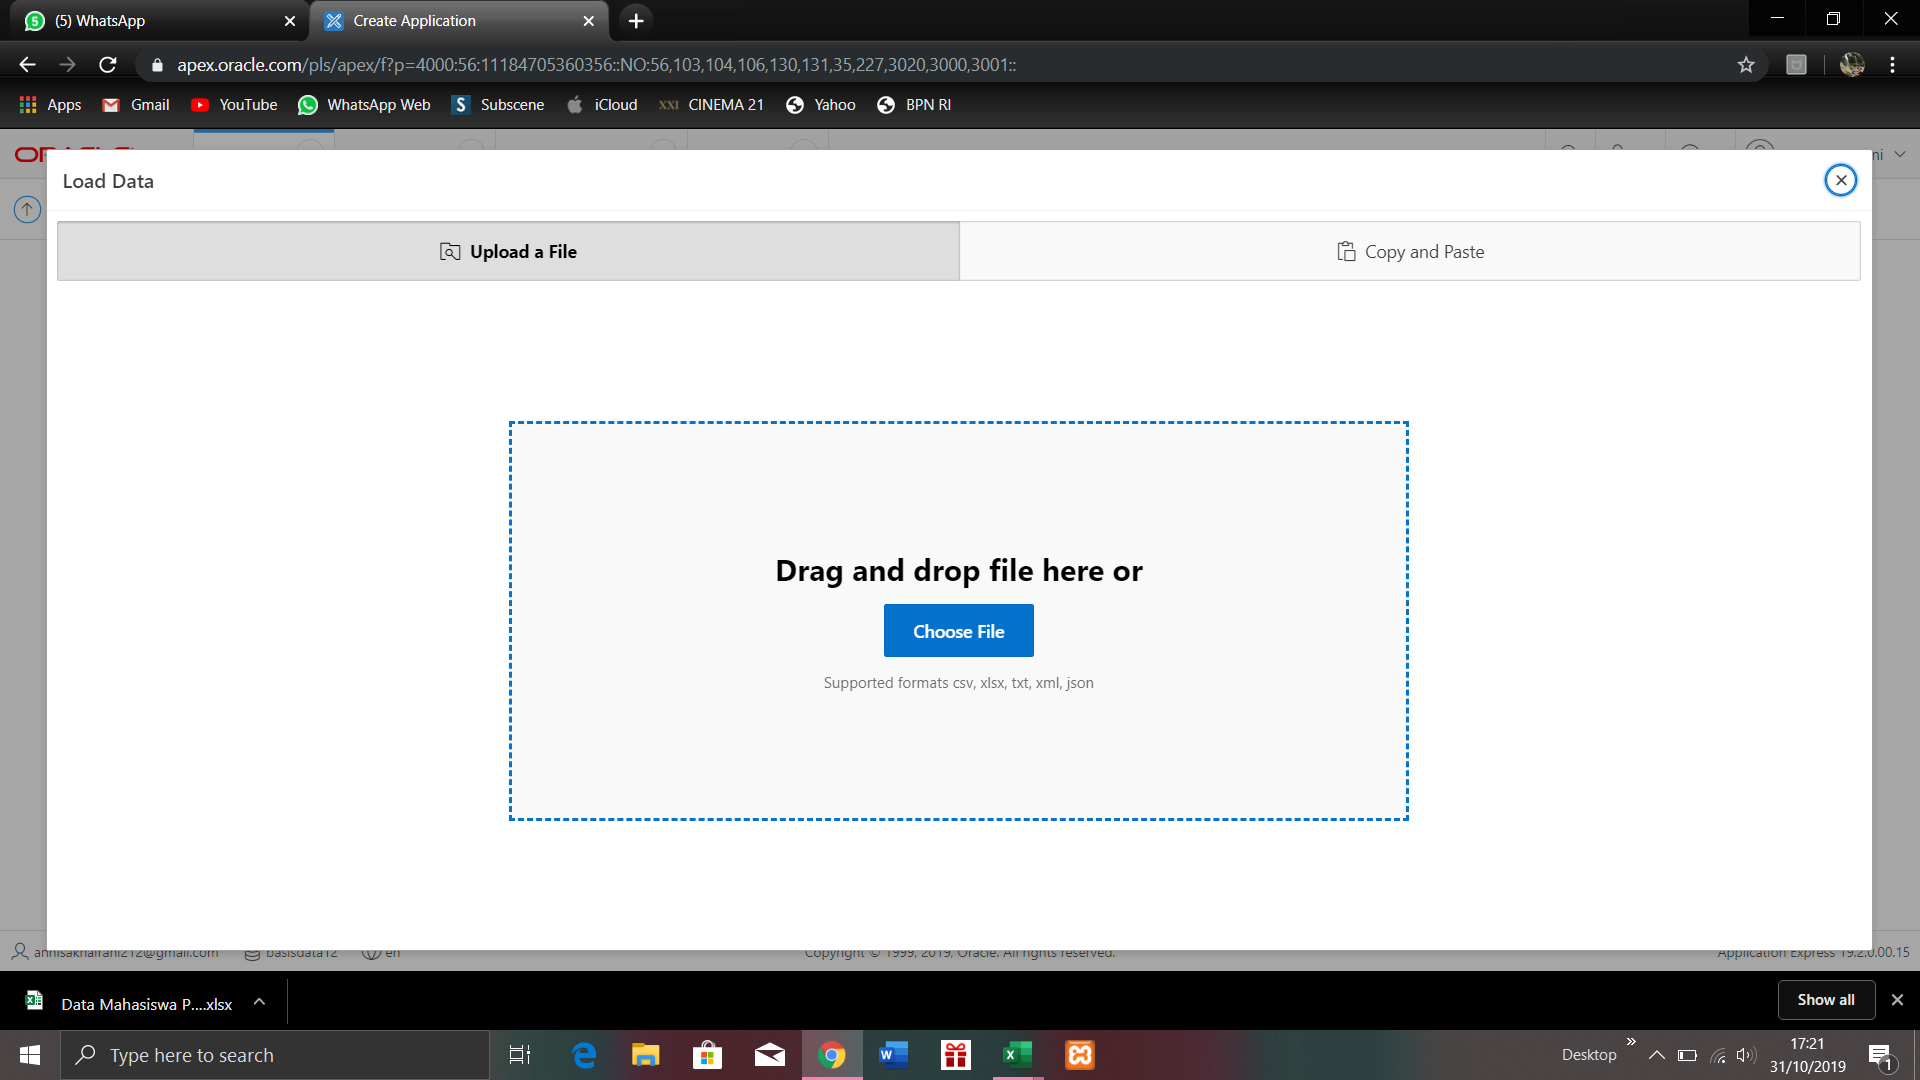
\includegraphics[width=8cm]{image/7.png}}
        \end{figure}
    \newpage \item Kemudian kita pilih choose file, lalu kita masukkan file excel kita ke dalam program tersebut terus kita tekan open
    \begin{figure}[h]
    \centerline{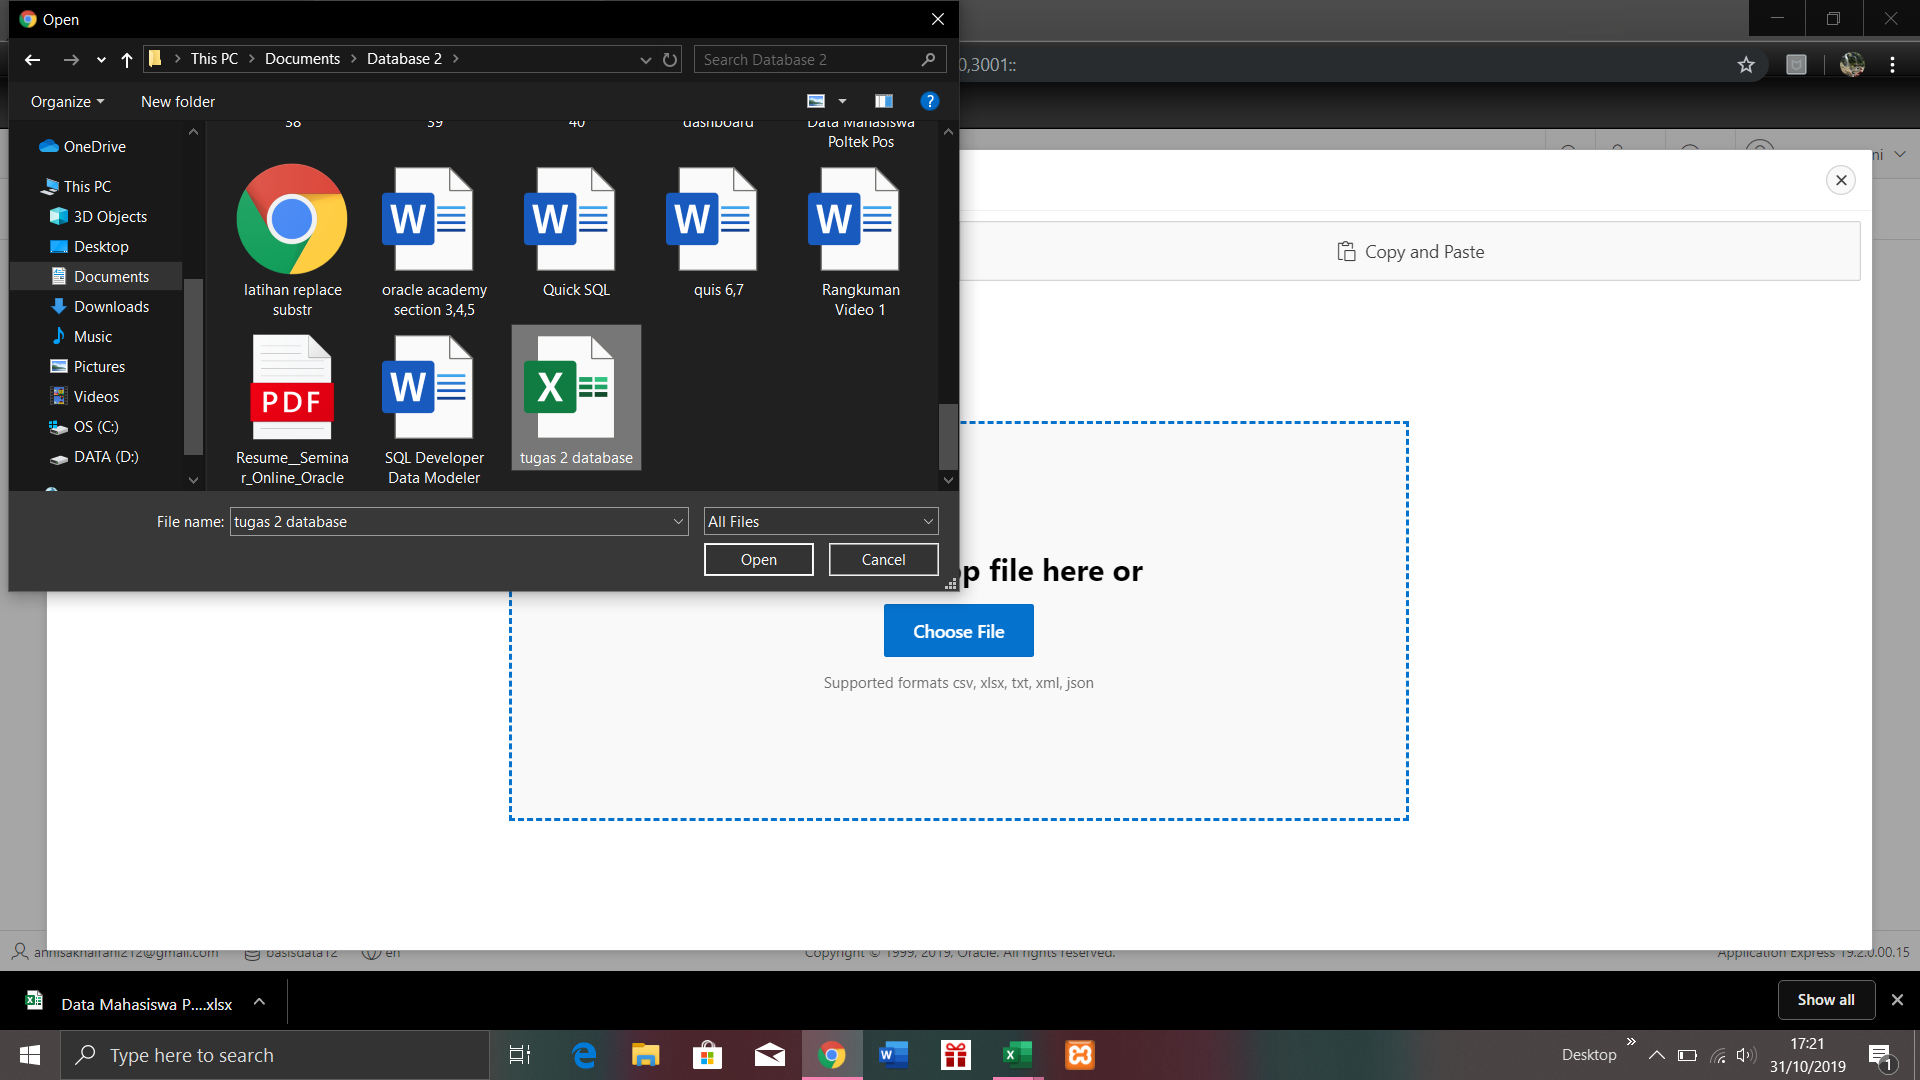
\includegraphics[width=8cm]{image/8.png}}
    \end{figure}
    \item Lalu kita masukkan tabel owner dan table ke dalam load data
    \begin{figure}[h]
    \centerline{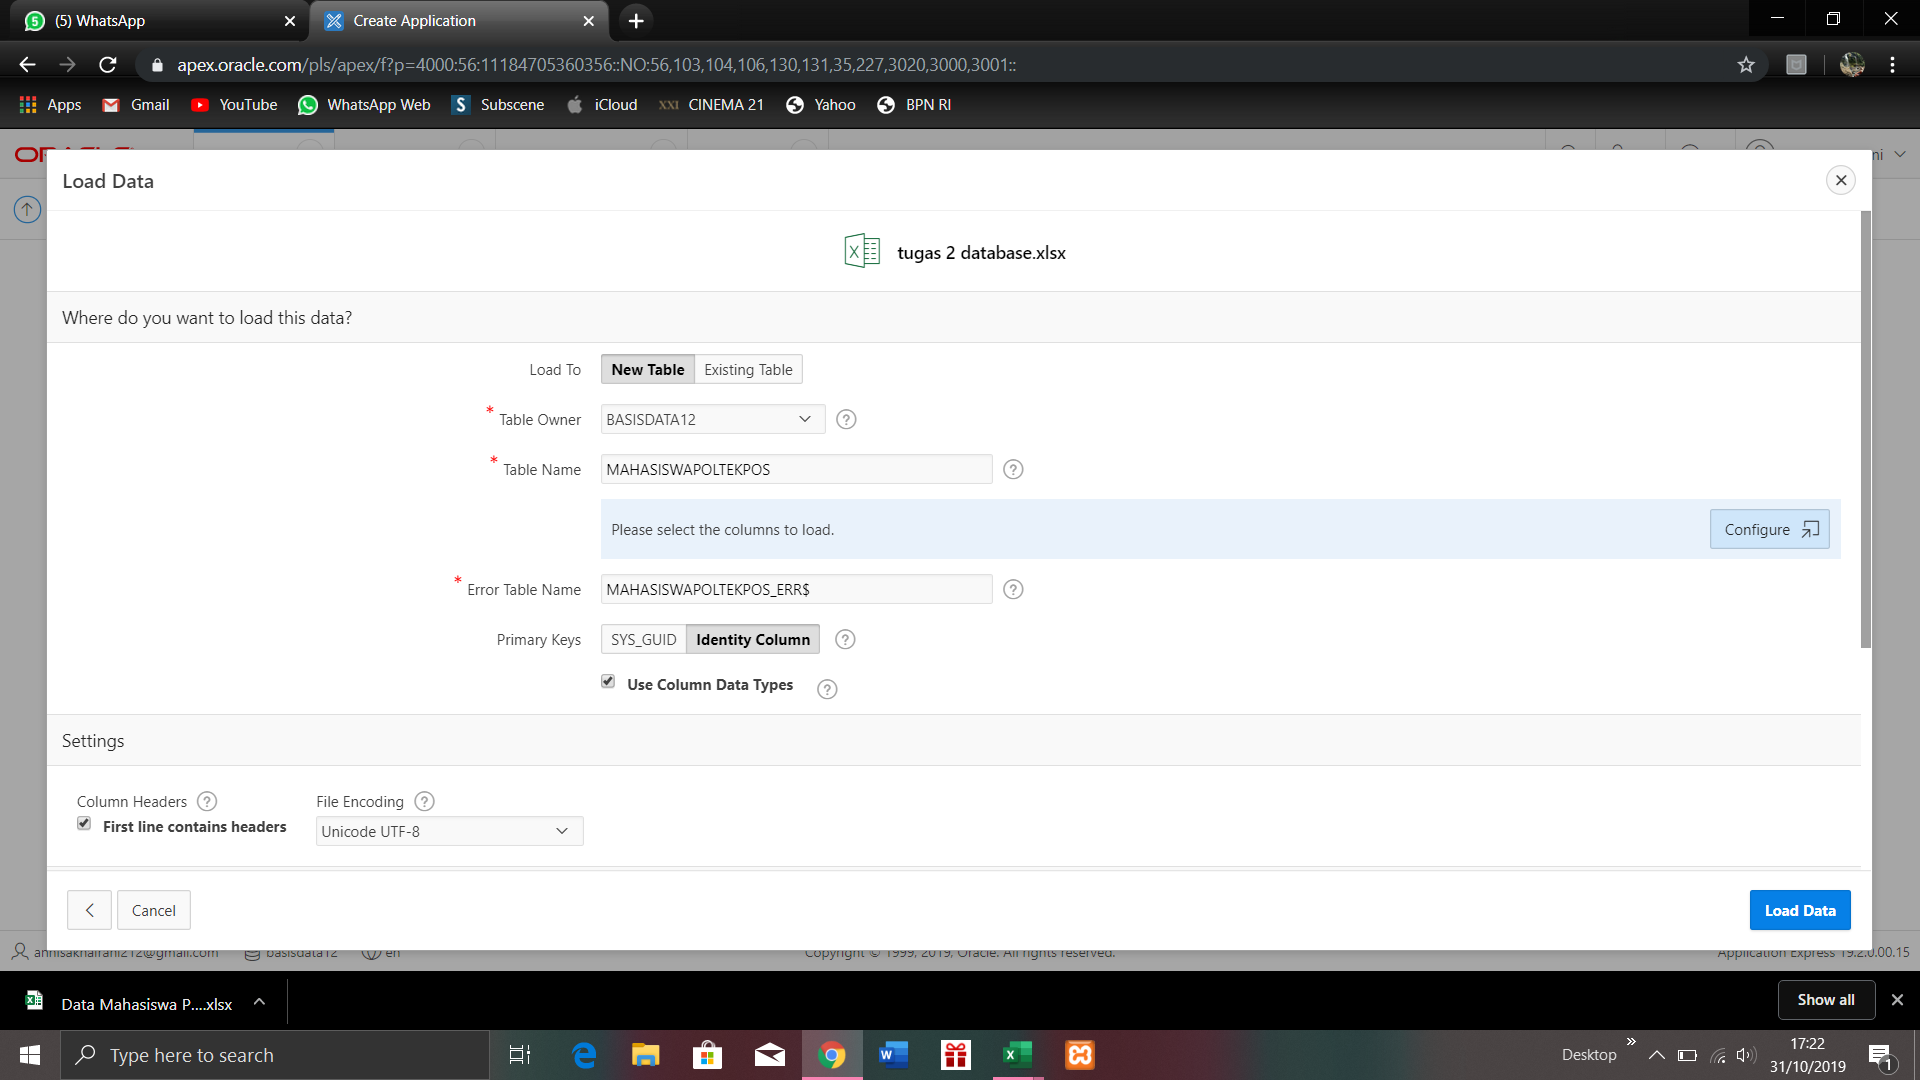
\includegraphics[width=8cm]{image/9.png}}
    \end{figure}
   \newpage \item Setelah itu apabila kita ingin melihat prievew kita turun ke bawah 
    \begin{figure}[h]
    \centerline{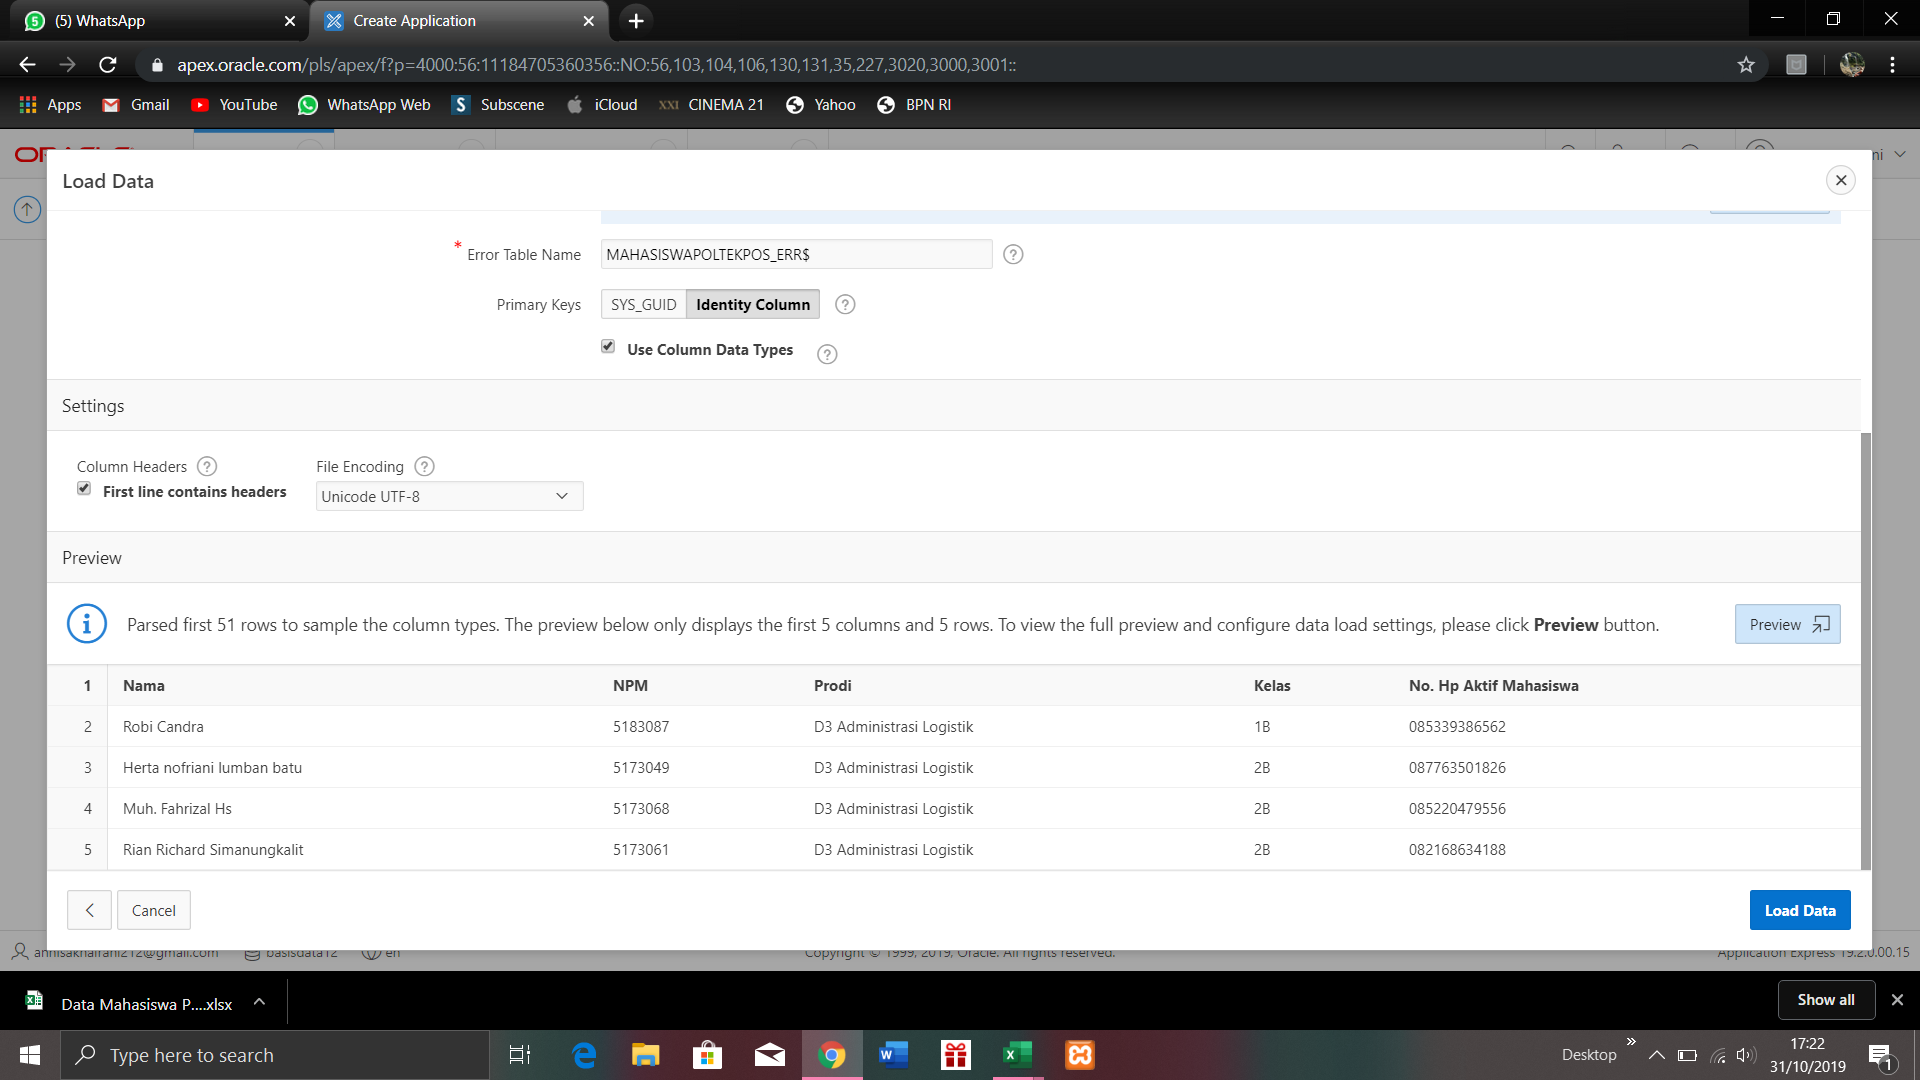
\includegraphics[width=8cm]{image/10.png}}
    \end{figure}
    \item Kemudian kita tekan preview 
    \begin{figure}[h]
    \centerline{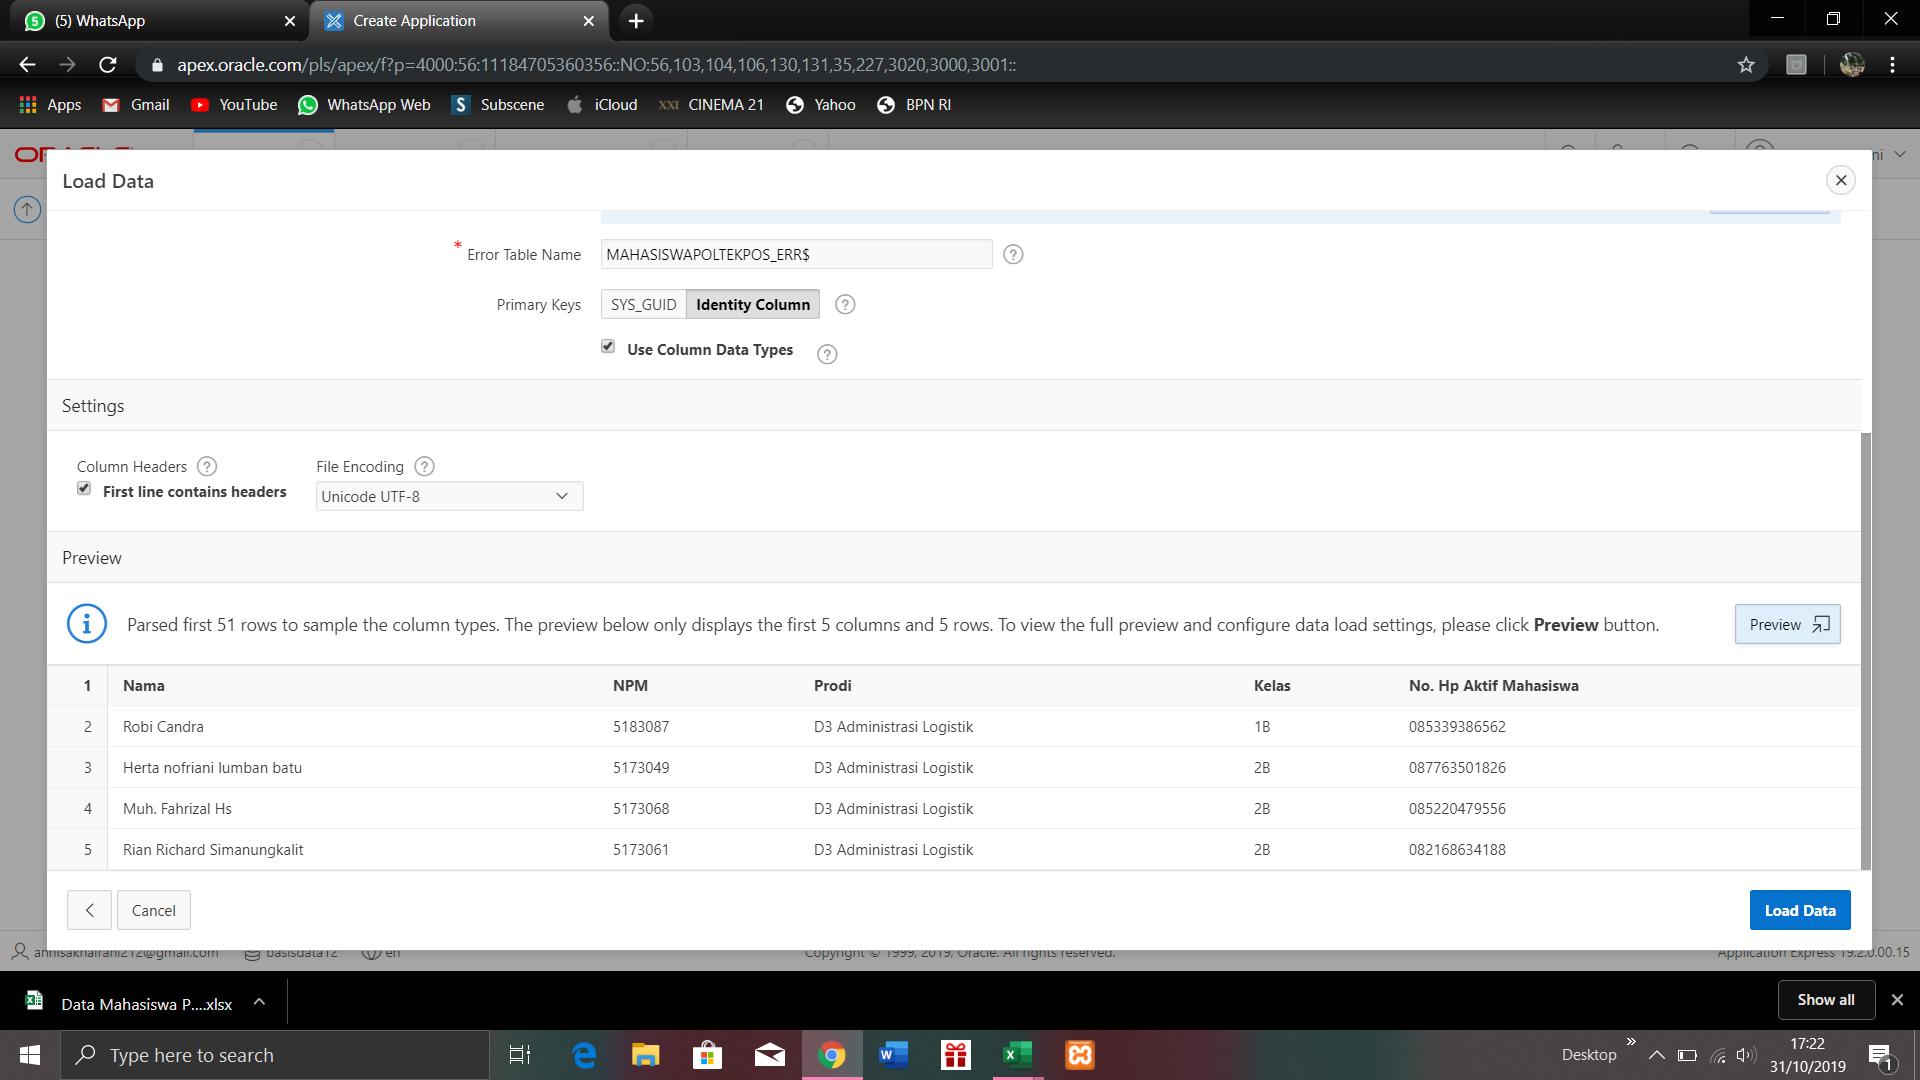
\includegraphics[width=8cm]{image/11.png}}
    \end{figure}
    \item Lalu akan muncul tampilan seperti dibawah ini
    \begin{figure}[h]
    \centerline{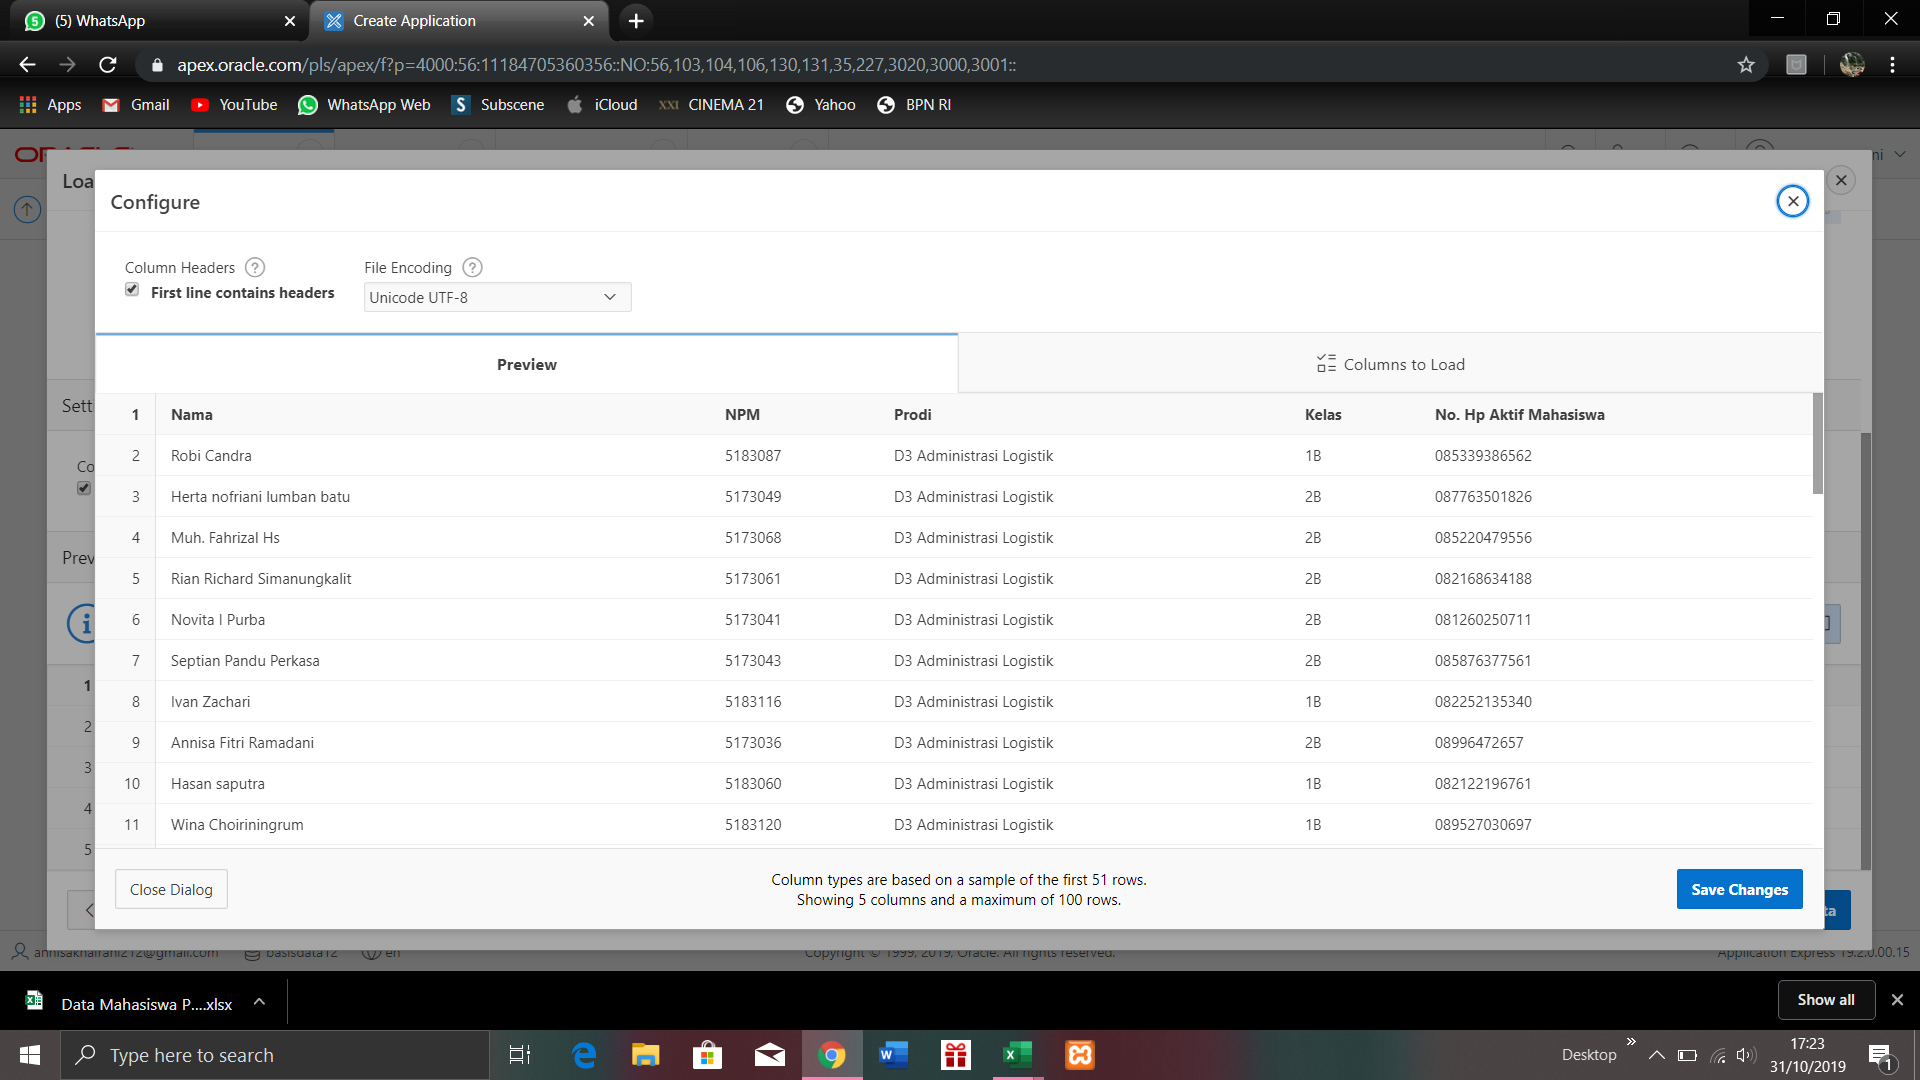
\includegraphics[width=8cm]{image/12.png}}
    \end{figure}
    \newpage\item Setelah itu kita pilih save changes
    \begin{figure}[h]
     \centerline{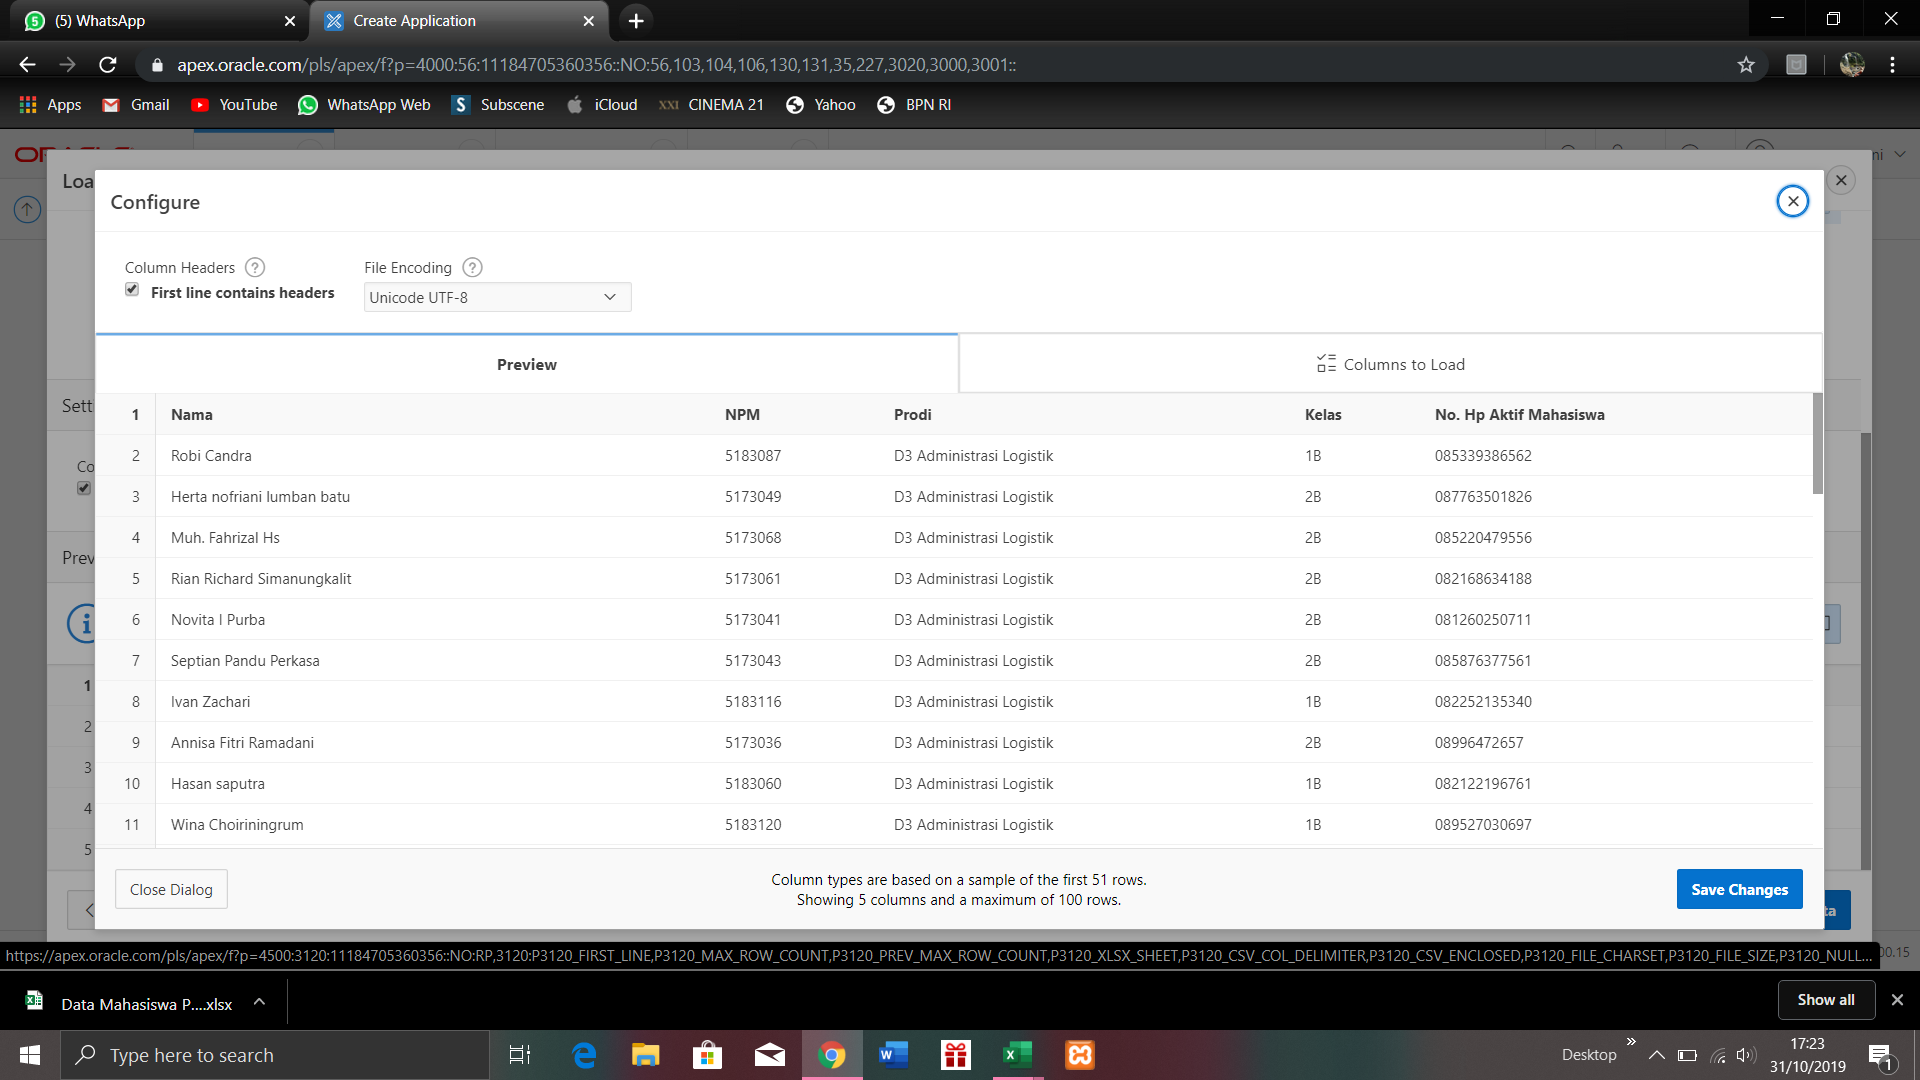
\includegraphics[width=8cm]{image/13.png}}
    \end{figure}
   \newpage \item Lalu akan muncul tampilan seperti dibawah ini
    \begin{figure}[h]
     \centerline{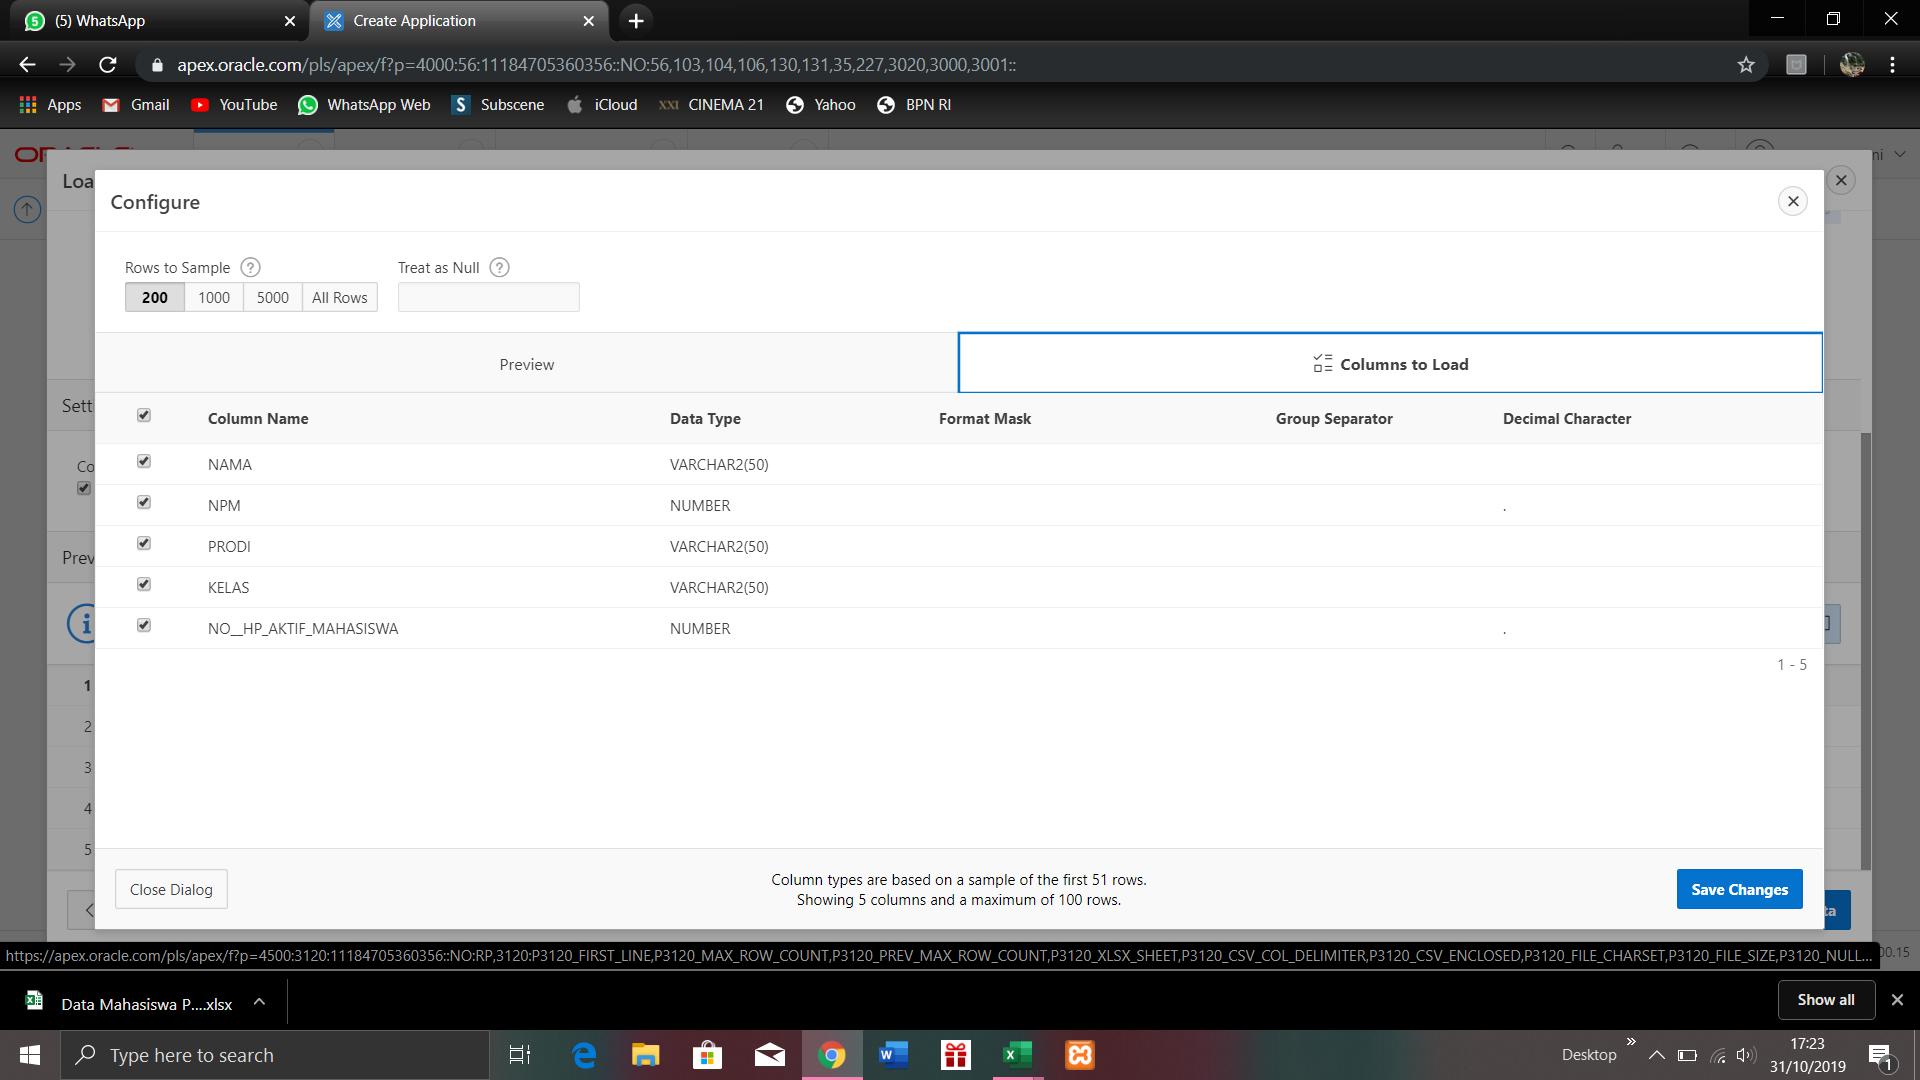
\includegraphics[width=8cm]{image/14.png}}
    \end{figure}
    \item Setelah itu kita pilih save changes lagi lalu akan muncul tampilan seperti ini,Kemudian kita pilih create application
    \begin{figure}[h]
    \centerline{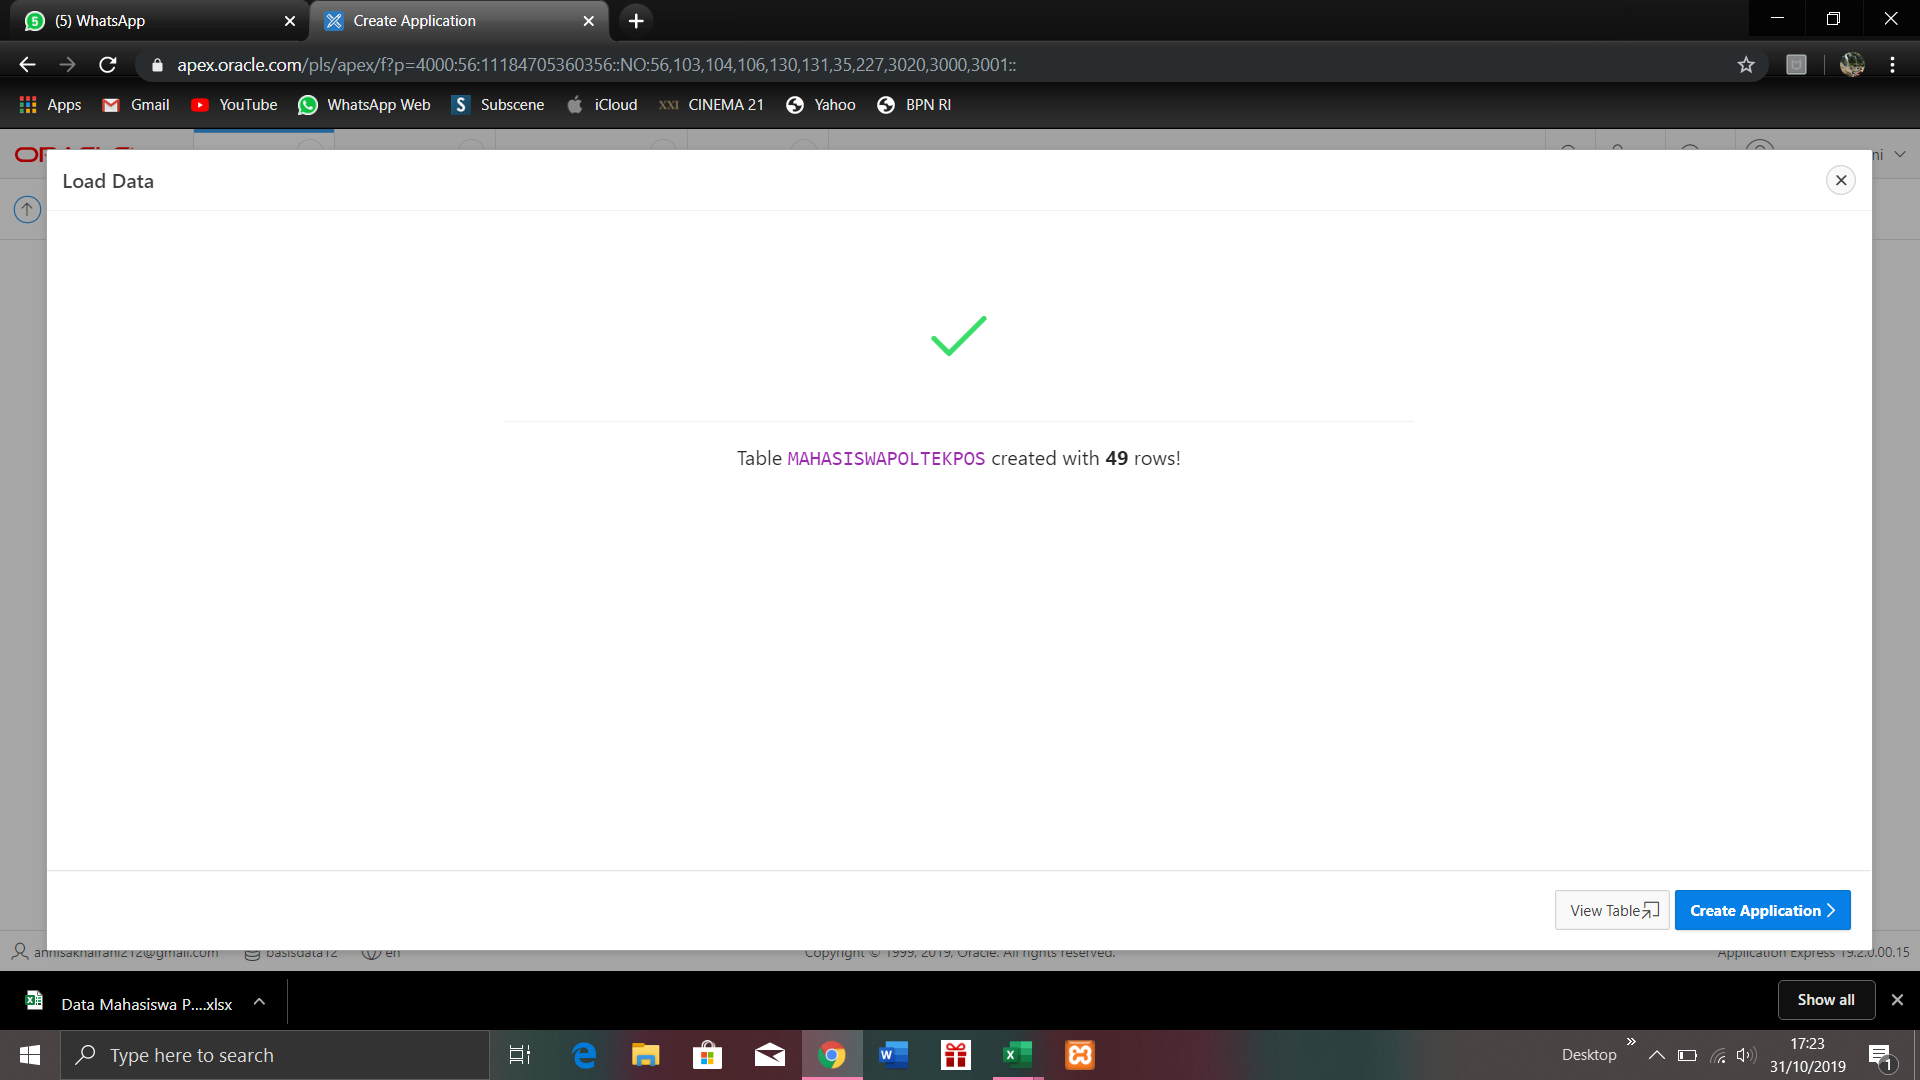
\includegraphics[width=8cm]{image/15.png}}
    \end{figure}
    \newpage \item Kemudian kita pilih create application dan akan muncul tampilan seperti dibawah ini
    \begin{figure}[h]
    \centerline{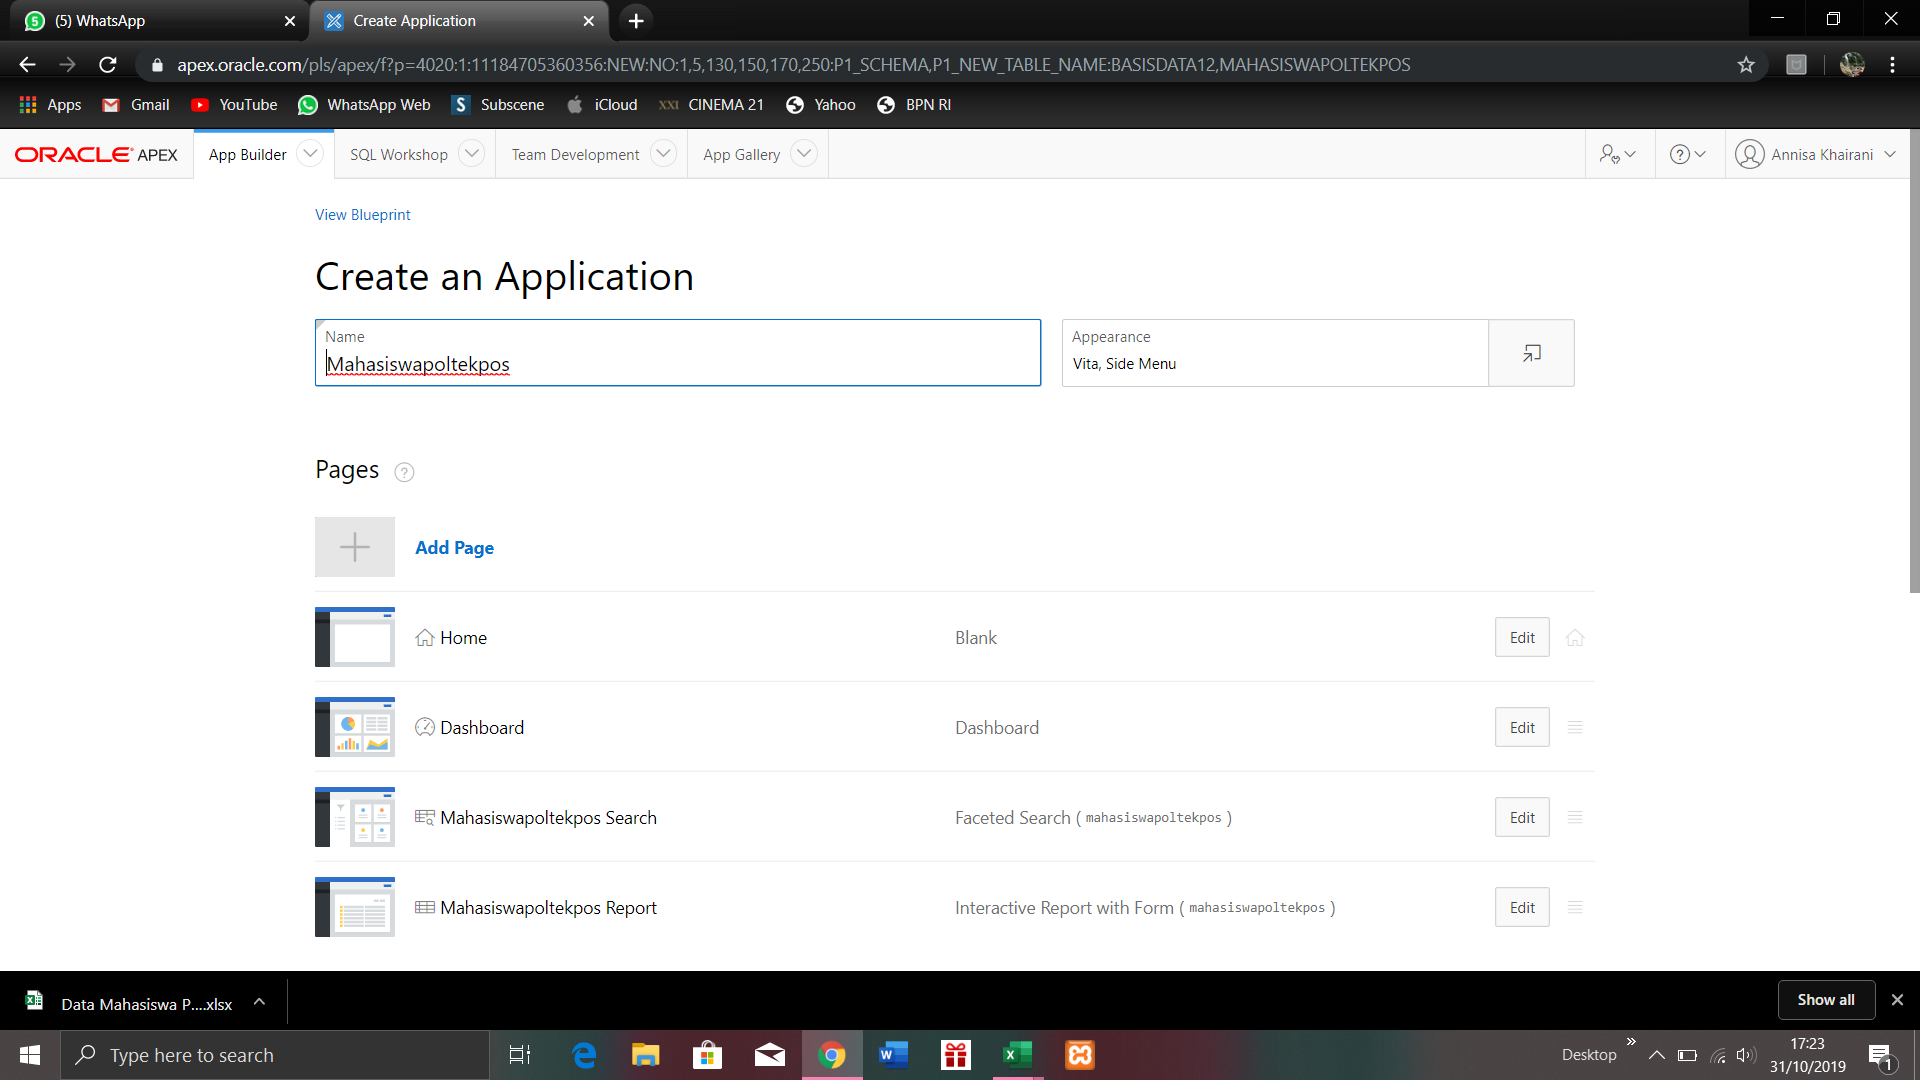
\includegraphics[width=8cm]{image/16.png}}
    \end{figure}
    \item Lalu kita pilih create application kembali
    \begin{figure}[h]
    \centerline{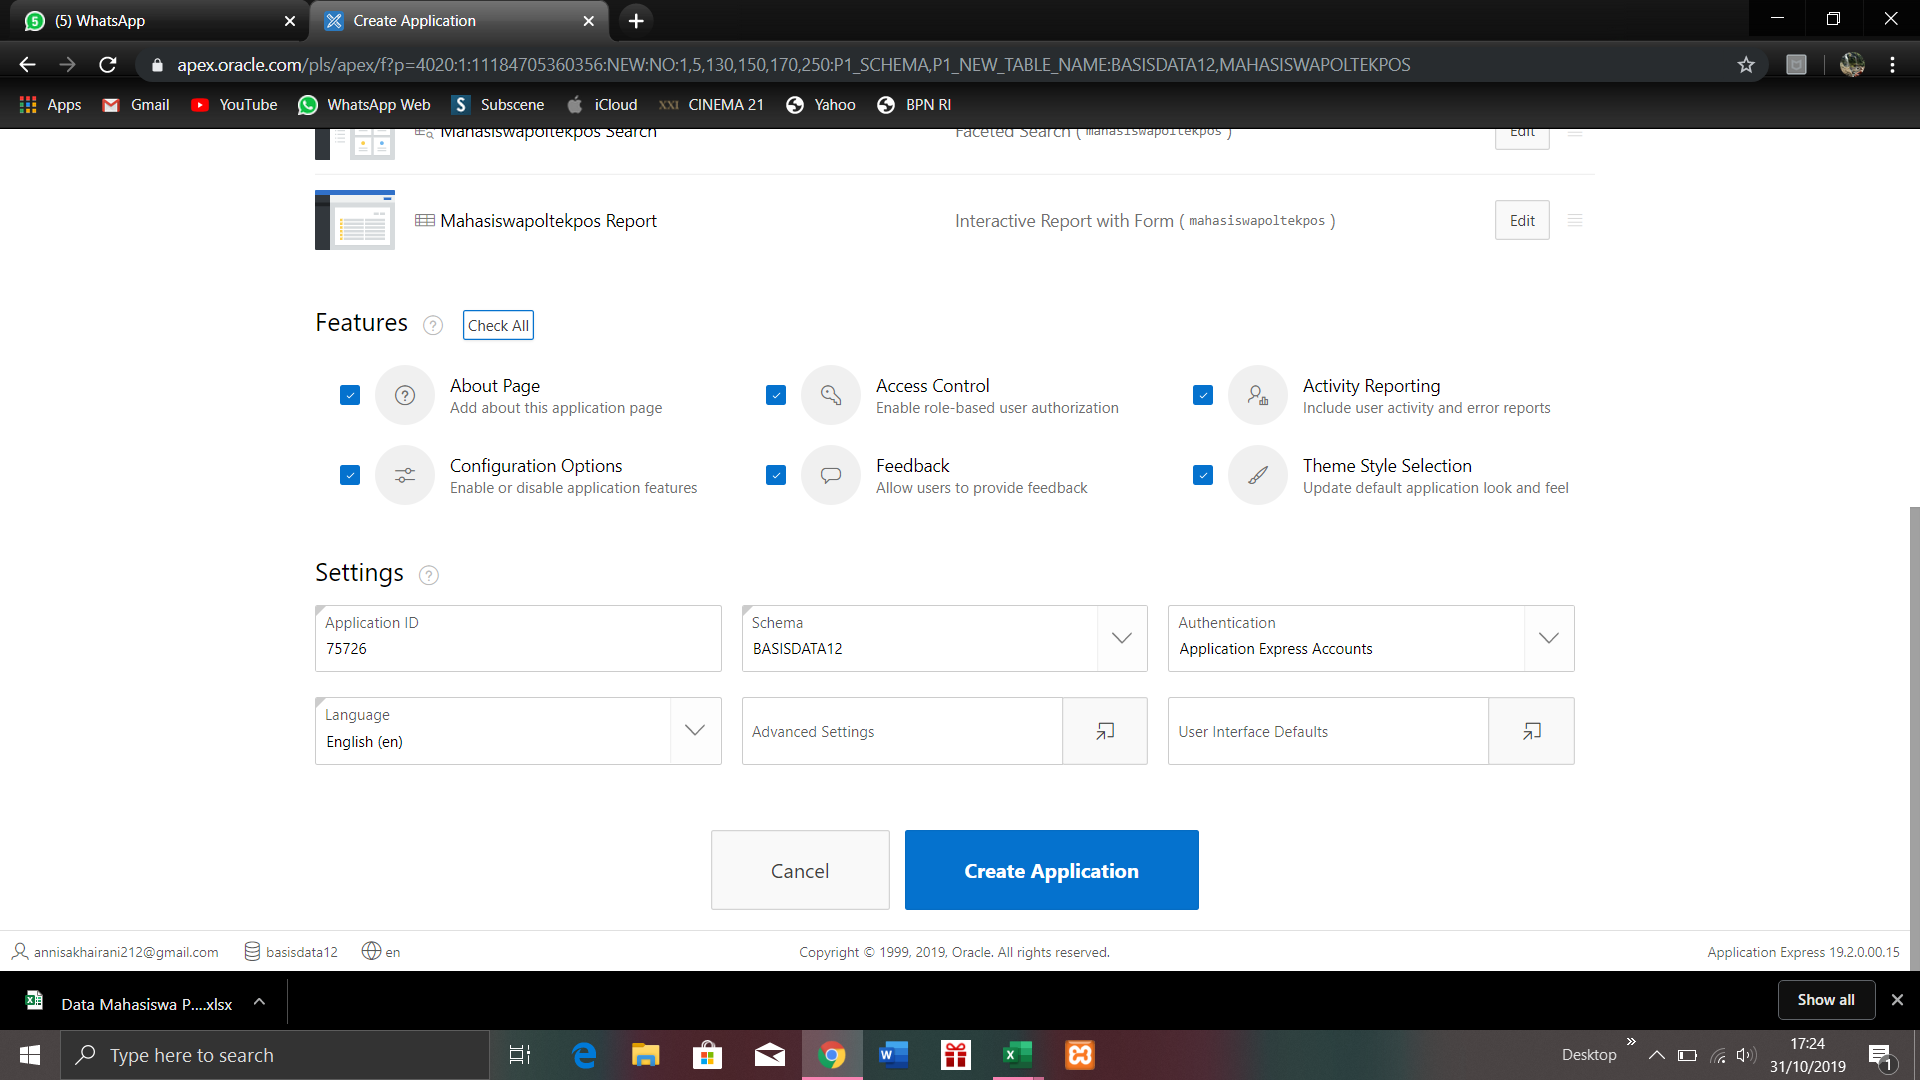
\includegraphics[width=8cm]{image/17.png}}
    \end{figure}
    \newpage\item Setelah itu kita pilih create application tersebut maka akan muncul tampilan loading
    \begin{figure}[h]
     \centerline{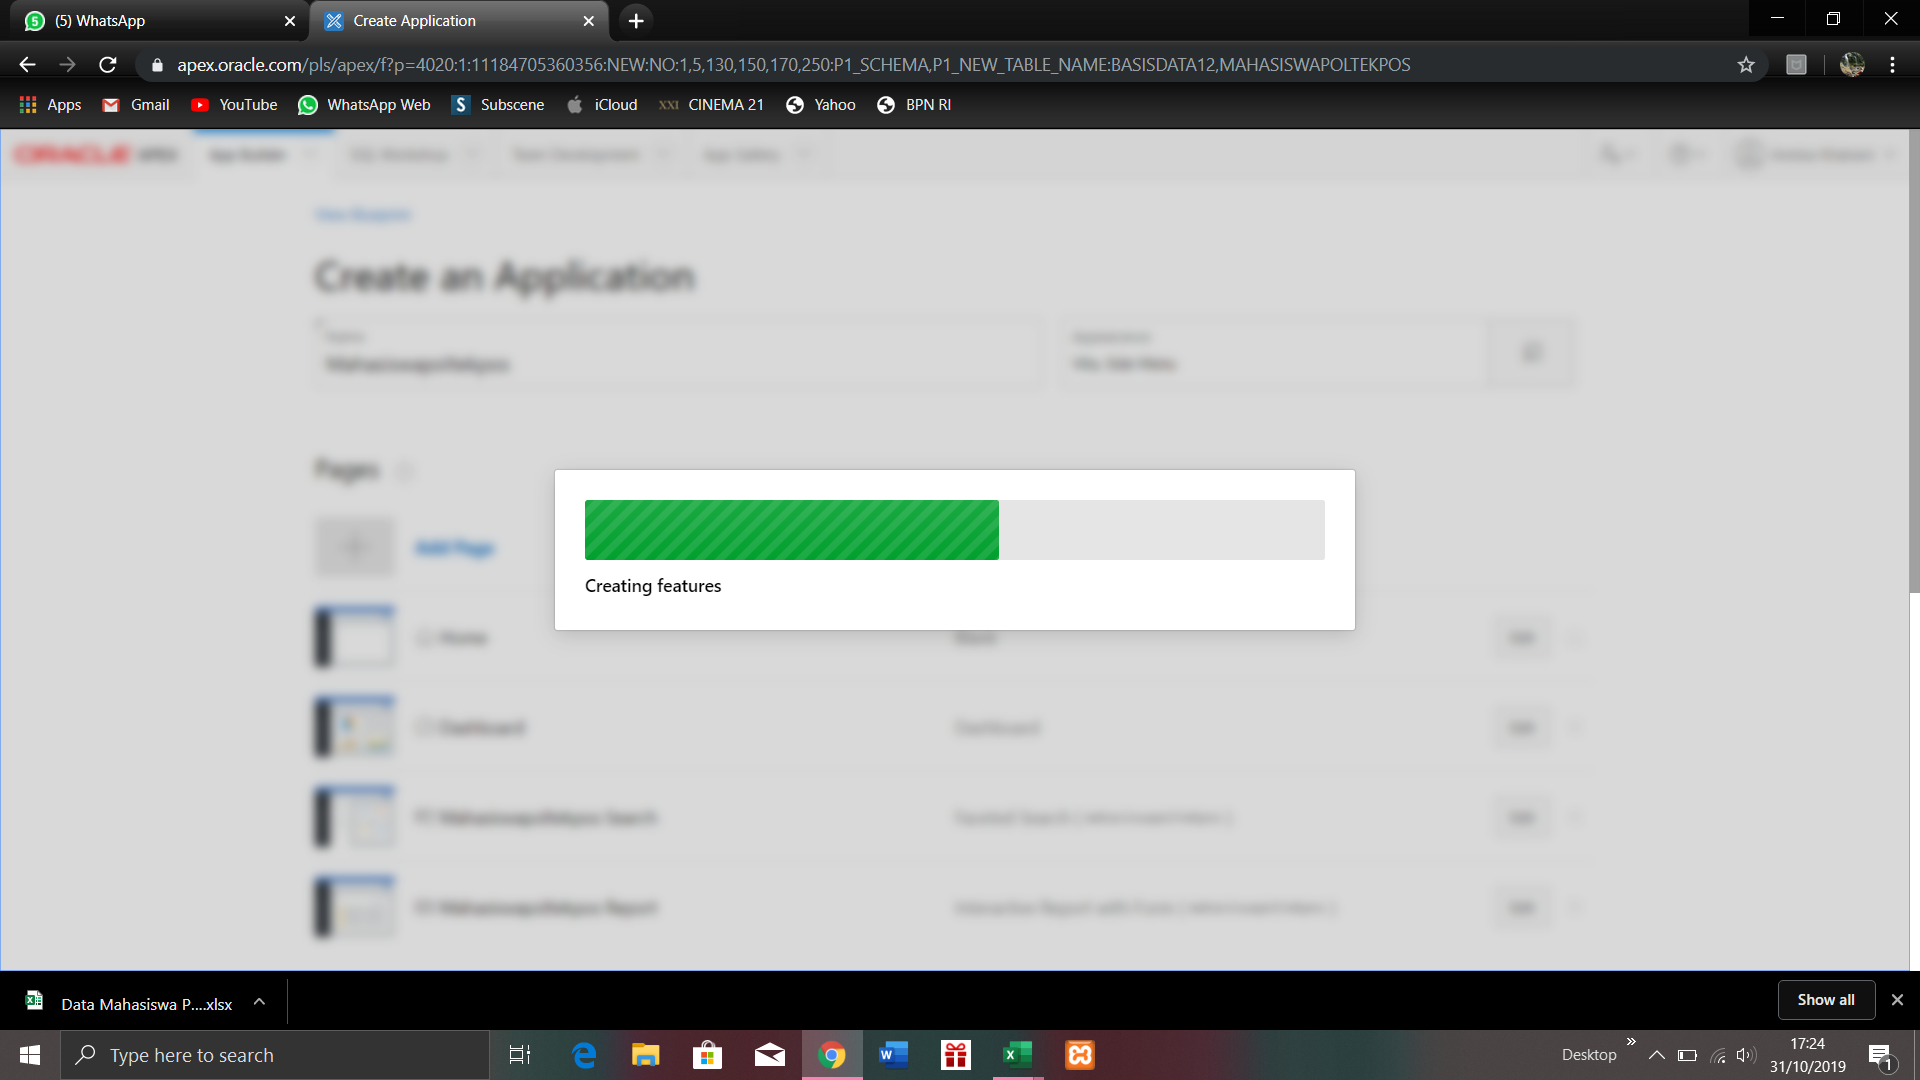
\includegraphics[width=8cm]{image/18.png}}
    \end{figure}
    \item Setelah loading nya selesai akan muncul tampilan seperti dibawah ini
    \begin{figure}[h]
    \centerline{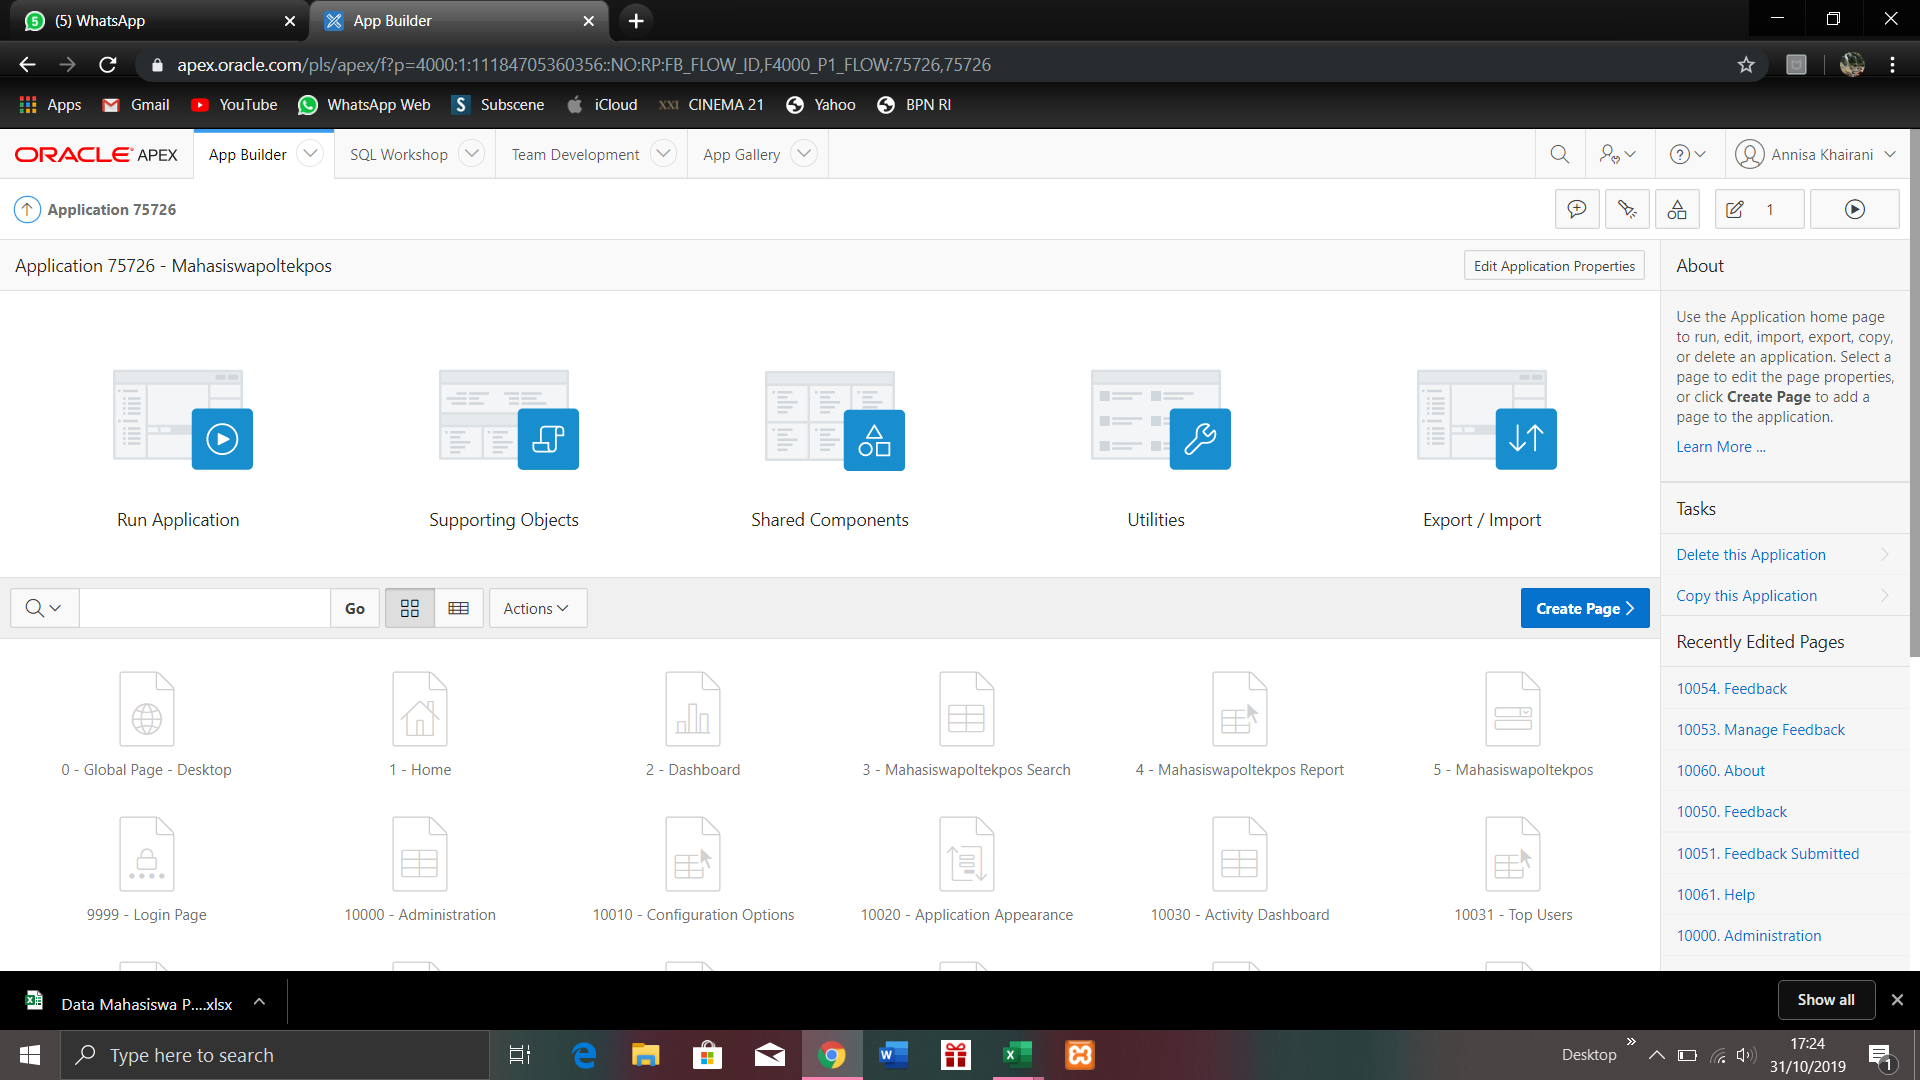
\includegraphics[width=8cm]{image/19.png}}
    \end{figure}
    \item Lalu kita pilih Run Application
    \begin{figure}[h]
    \centerline{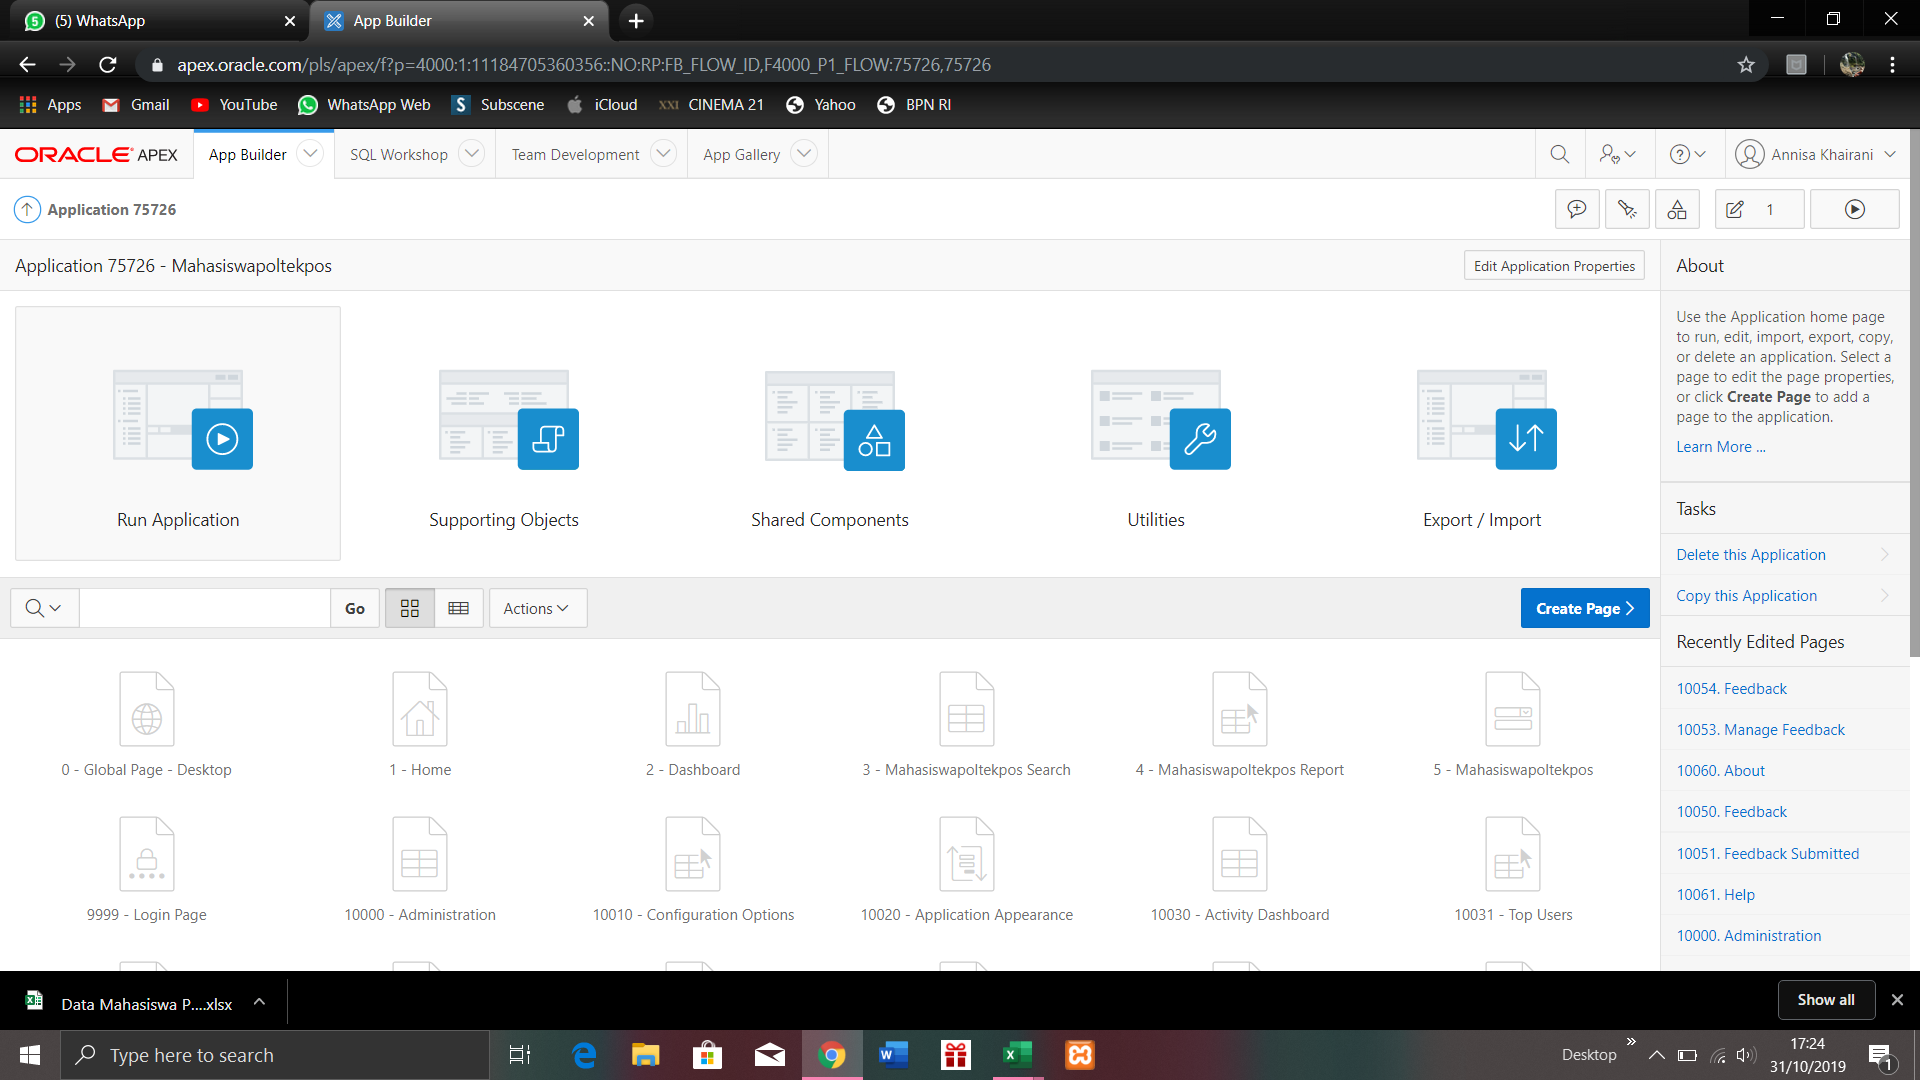
\includegraphics[width=8cm]{image/20.png}}
    \end{figure}
    \newpage \item Kemudian akan muncul tampilan seperti dibawah ini, Lalu masukkan username dan password
    \begin{figure}[h]
    \centerline{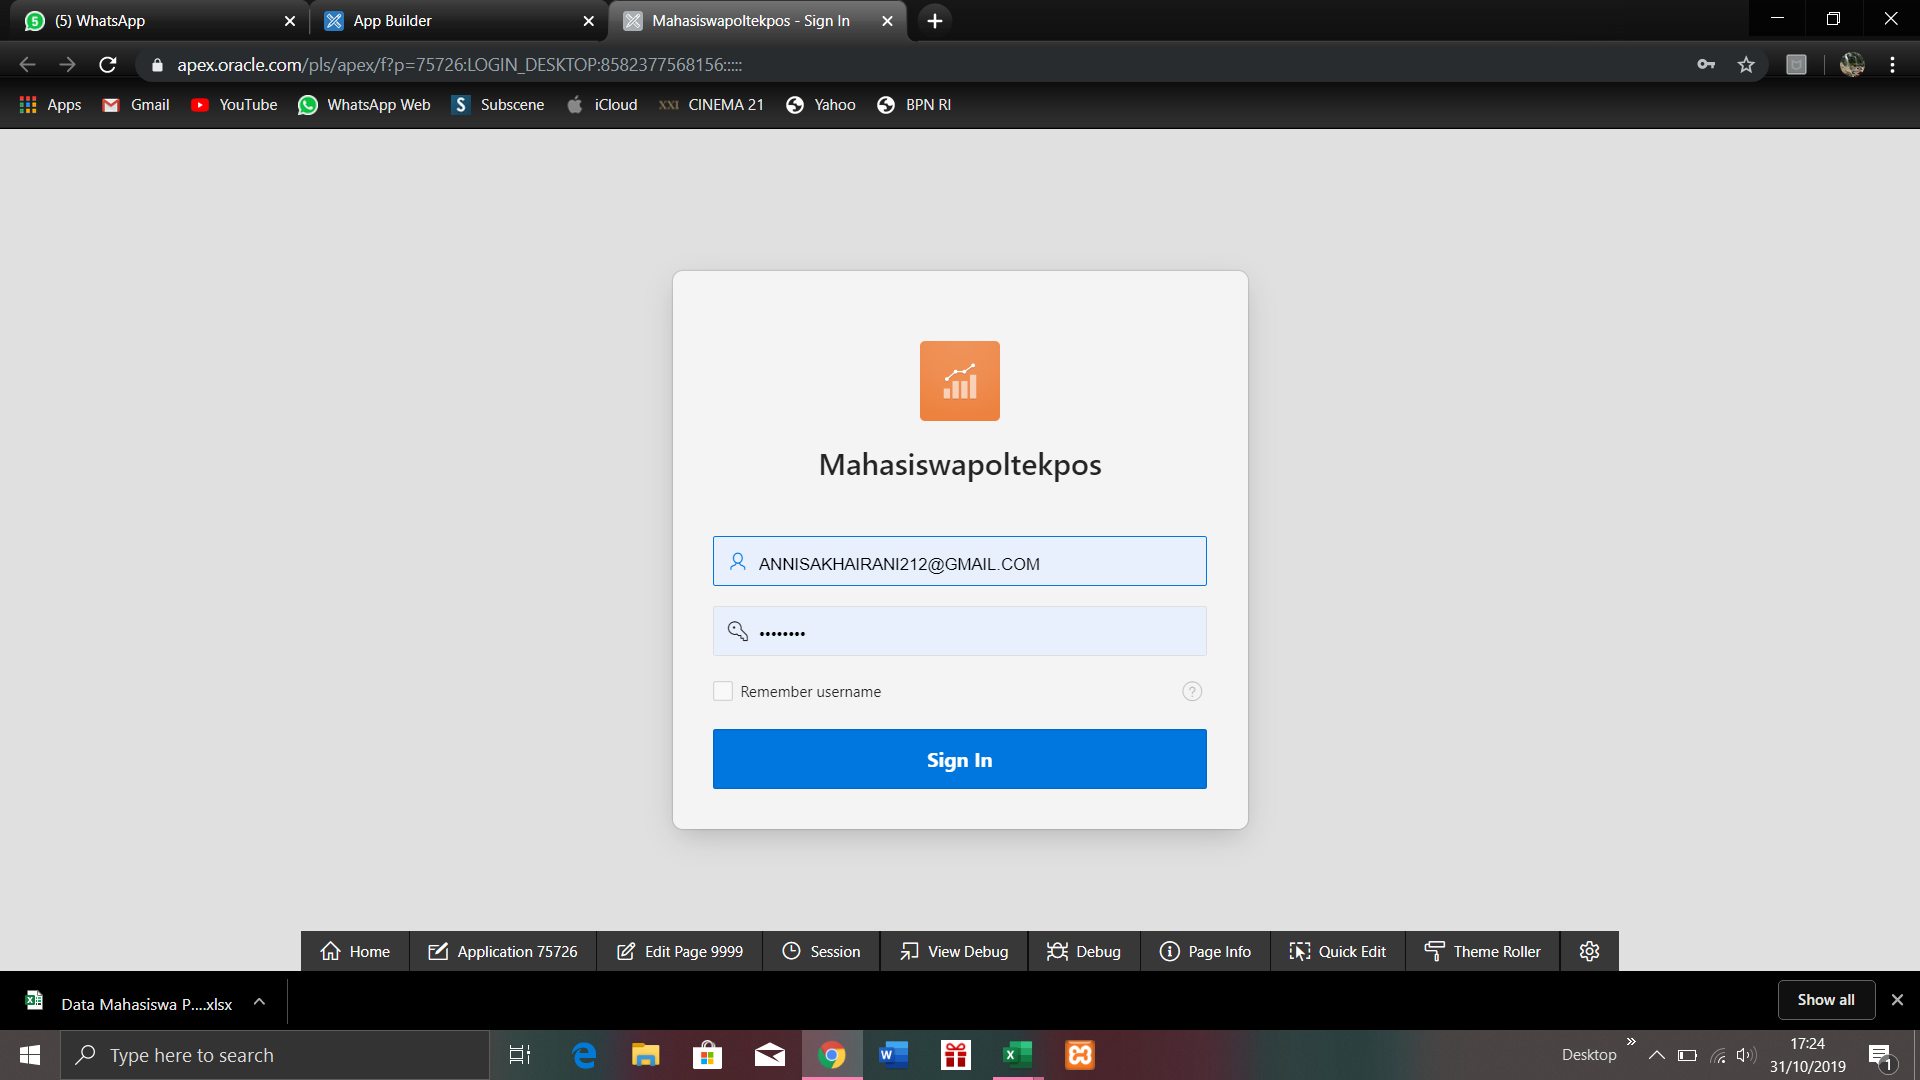
\includegraphics[width=8cm]{image/21.png}}
    \end{figure}
    \newpage \item Setelah kita masukkan password akan muncul tampilan dibawah ini yaitu Dashboard,Mahasiswapoltekpos Search dan Report
    \begin{figure}[h]
    \centerline{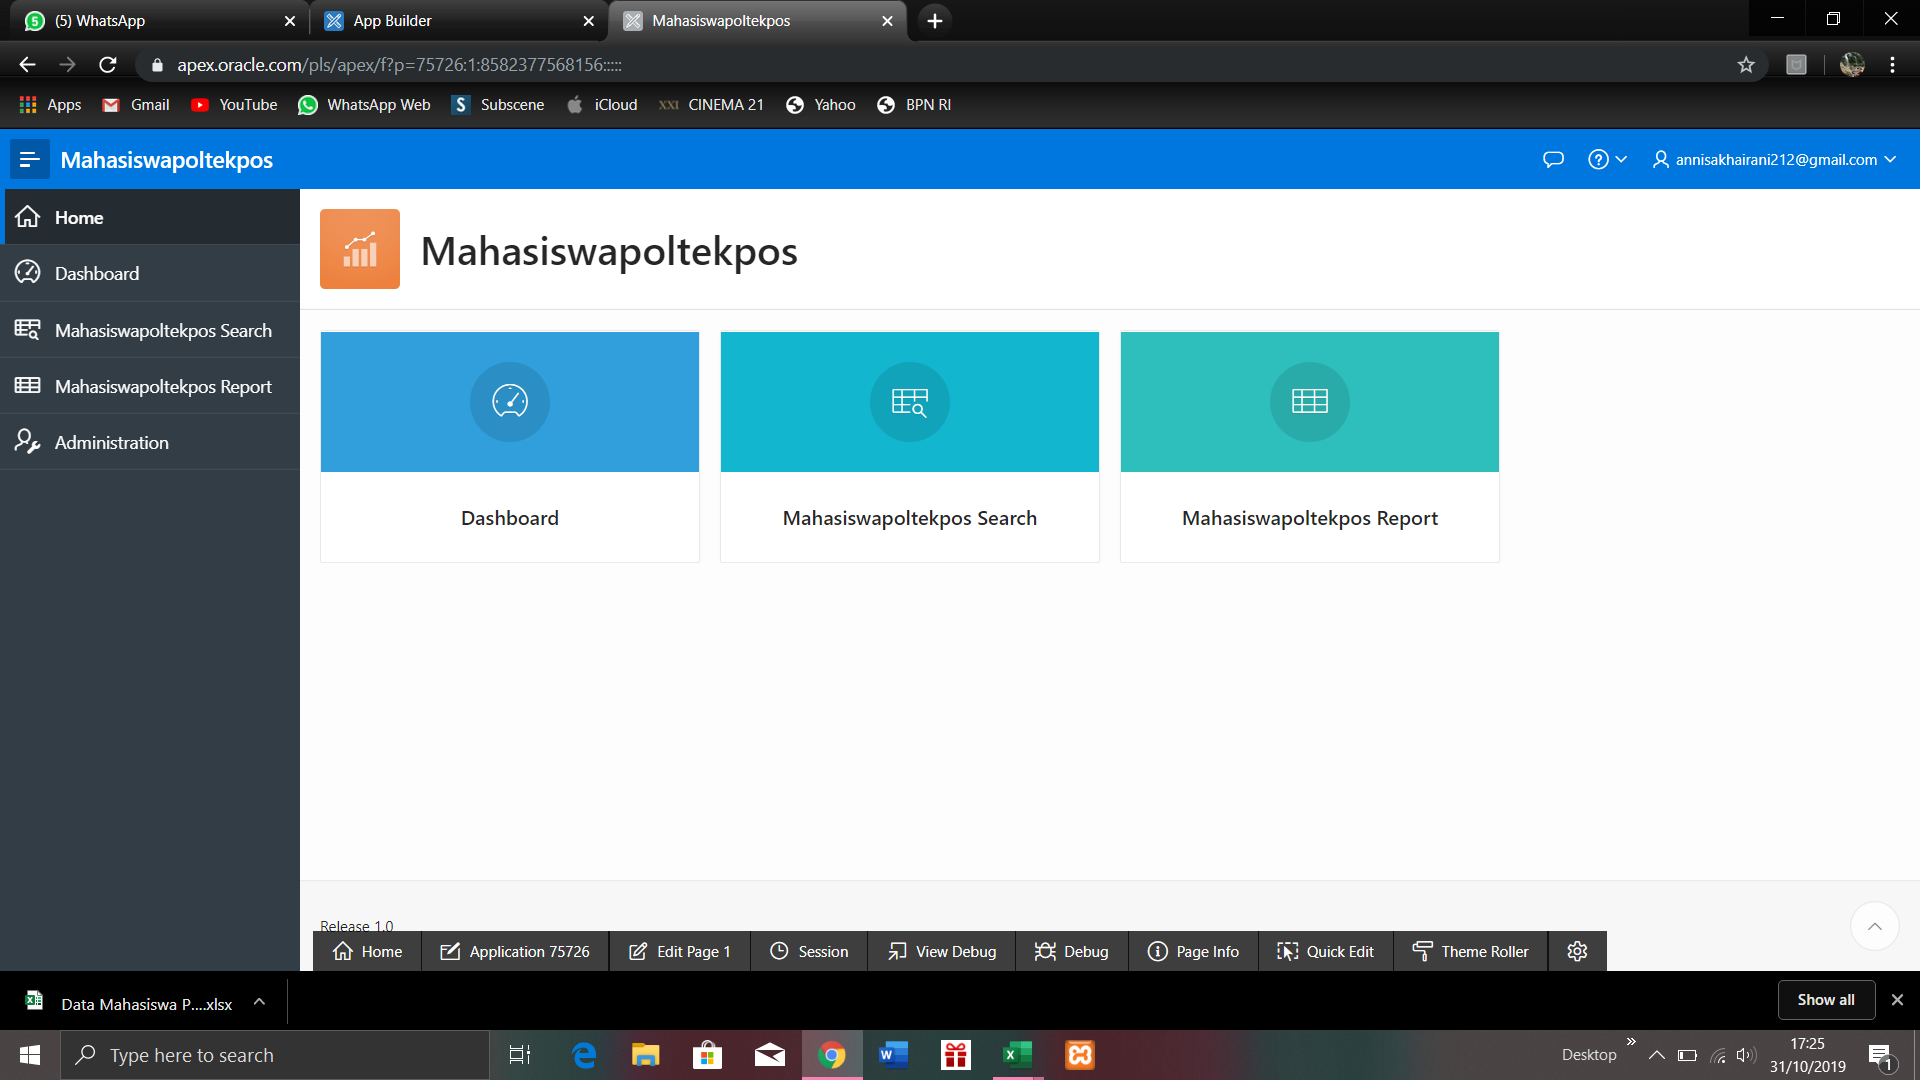
\includegraphics[width=8cm]{image/22.png}}
    \end{figure}
    \item Kemudian apabila kita ingin melihat tampilan dashboard kita klik tersebut
    \begin{figure}[h]
    \centerline{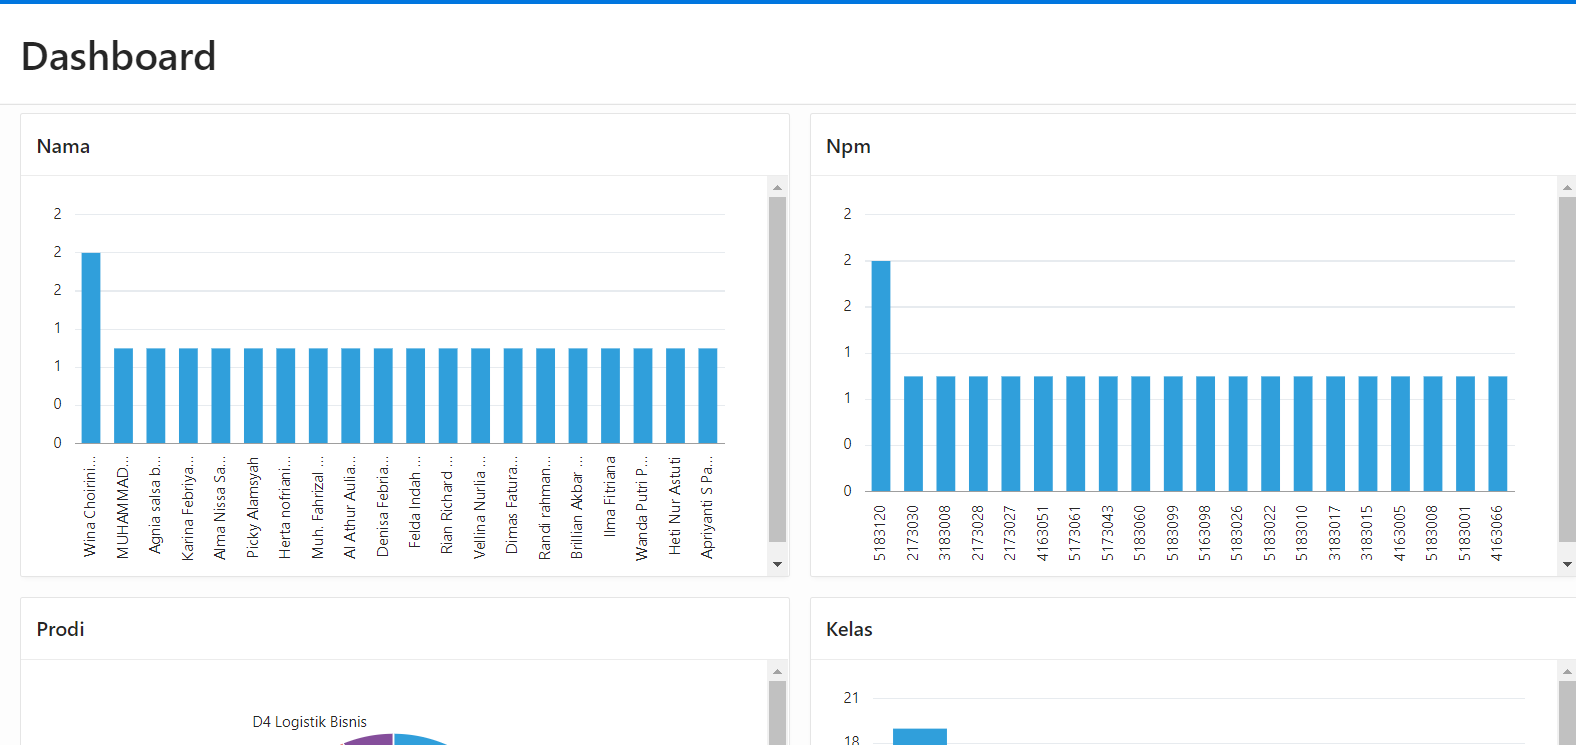
\includegraphics[width=8cm]{image/dashboard.PNG}}
    \end{figure}
    \item Lalu apabila kita ingin melihat tampilan administrasi kita klik maka akan muncul tampilan seperti ini
    \begin{figure}[h]
    \centerline{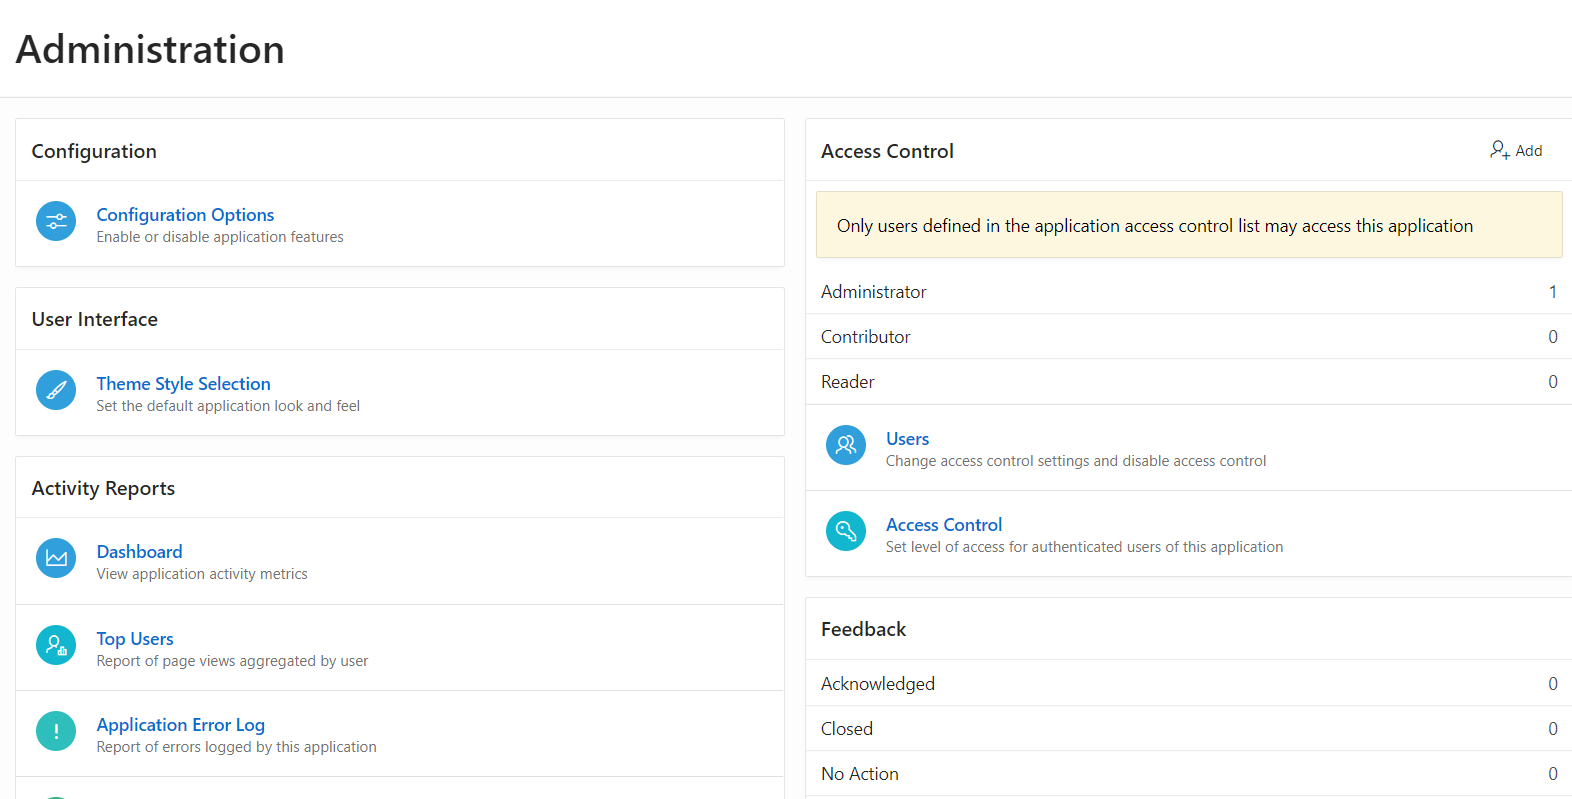
\includegraphics[width=8cm]{image/administrasi.PNG}}
    \end{figure}
    \newpage \item Apabila kita ingin melihat tampilan mahasiswa poltekpos search kita klik maka akan muncul tampilan dibawah ini
    \begin{figure}[h]
    \centerline{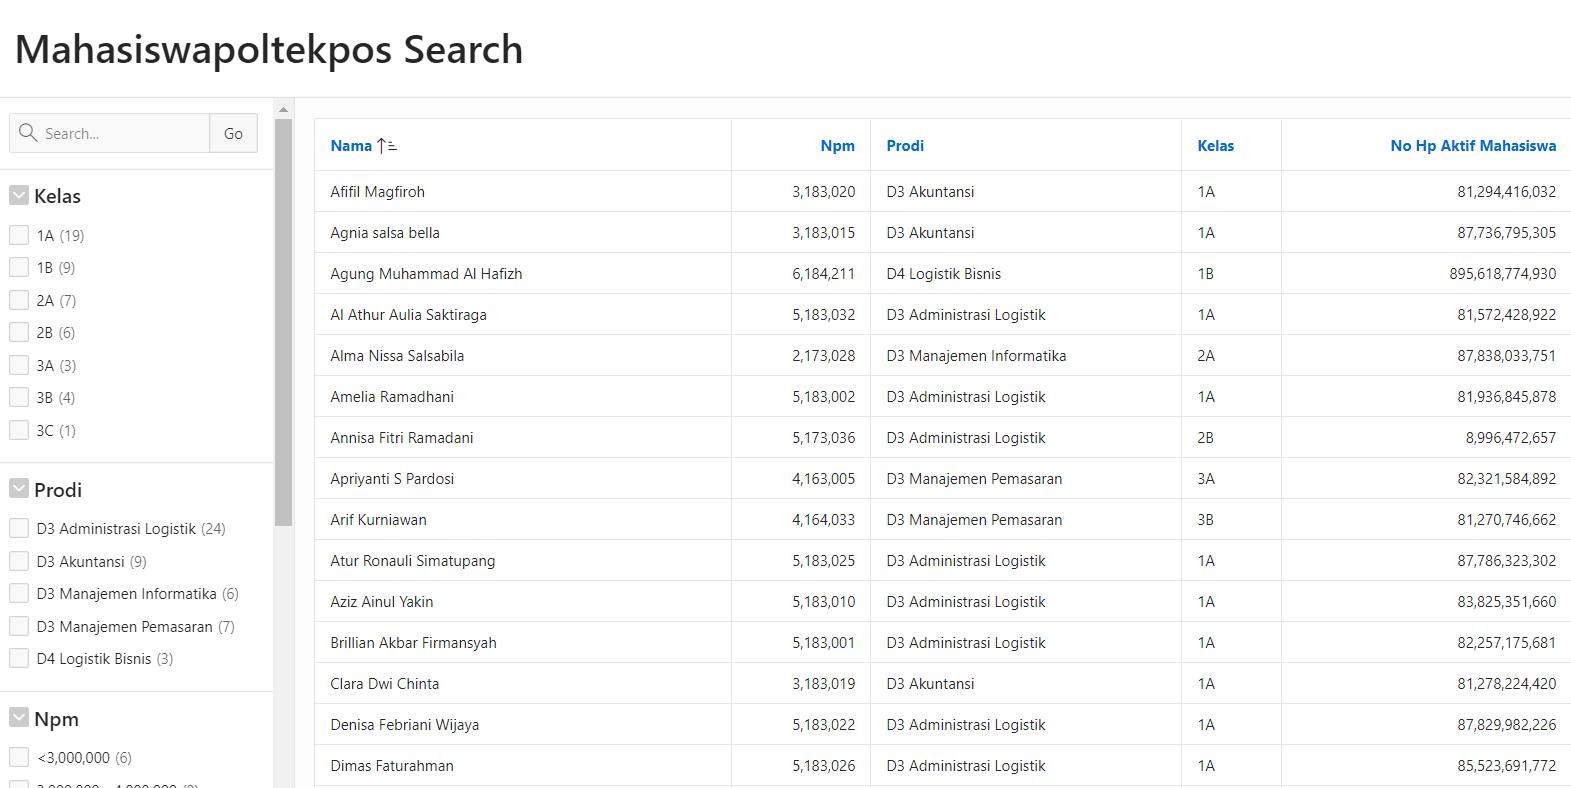
\includegraphics[width=8cm]{image/mahasiswapoltekpos.PNG}}
    \end{figure}
    \item Dan terakhir apabila kita ingin melihat tampilan mahasiswa report kita klik maka akan muncul tampilan dibawah ini
    \begin{figure}[h]
    \centerline{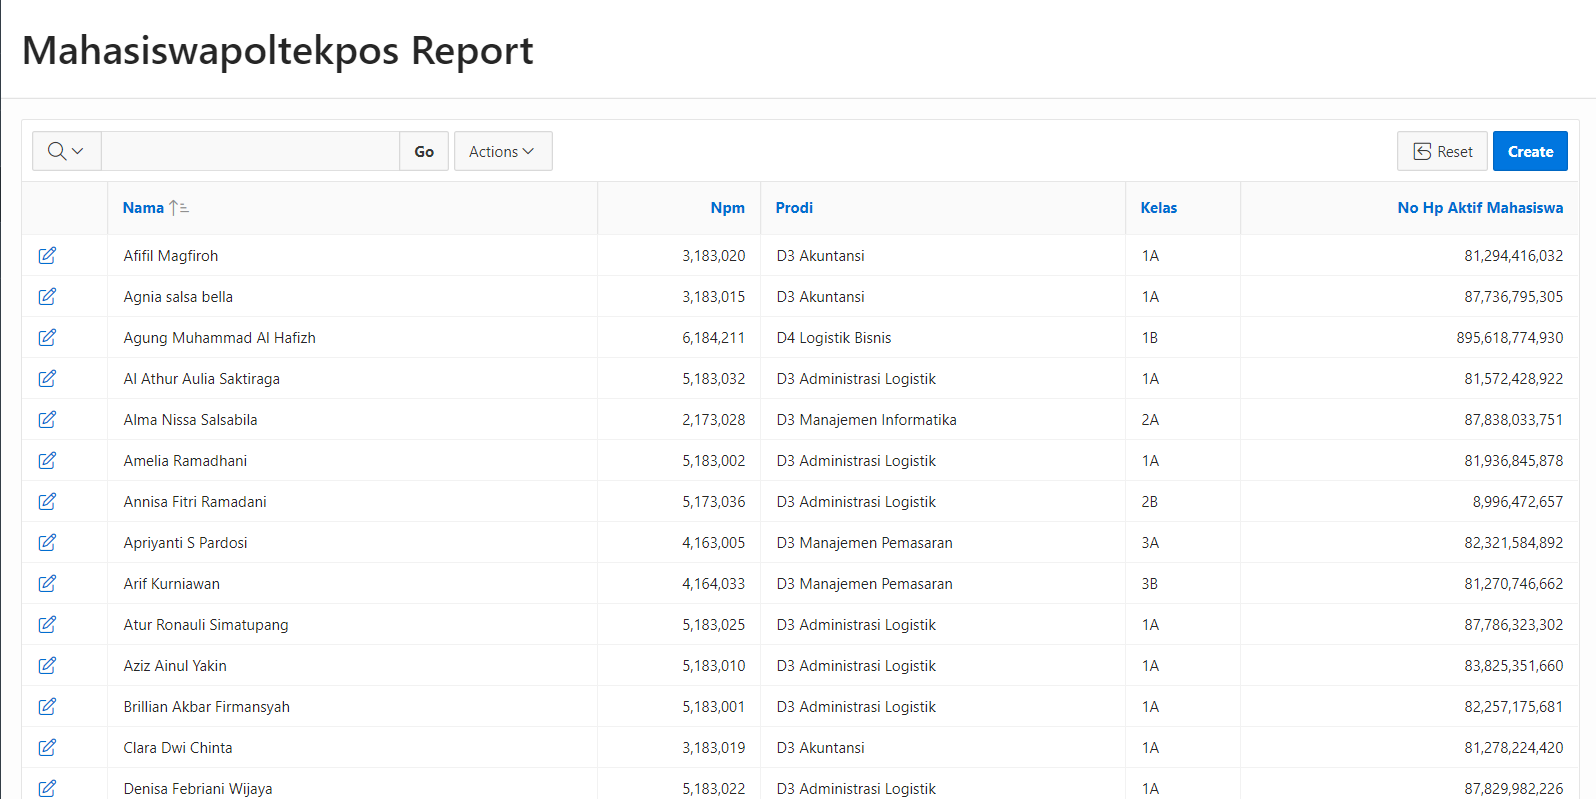
\includegraphics[width=8cm]{image/mahasiswareport.PNG}}
    \end{figure}
\end{enumerate}
\end{document}
